\documentclass[a4paper,10p]{report}

%Package math
\usepackage{amsmath}
\usepackage{amsfonts}
\usepackage{amssymb}

%Bibliographie
%\usepackage{biblatex}

%insérer des illustration
\usepackage{caption}
\usepackage{graphicx}

%convertion des caractères spéciaux type "é" + affichage de ces même carractères
\usepackage[utf8]{inputenc}
\usepackage[T1]{fontenc}

%"Francisé" le codage
\usepackage[french]{babel}
%éviter des conflit entre babel et les listing
\frenchbsetup{StandardLists=true}

%insérer de la couleur
\usepackage{xcolor}

%faire des listes
\usepackage{enumitem}

%Liens hyper texte
\usepackage{hyperref}
\hypersetup{
    colorlinks=true,
    linkcolor=brown,
    filecolor=blue,      
    urlcolor=blue,
    }

%Liens URL
\usepackage{url}

\usepackage[left=2cm,right=2cm,top=2cm,bottom=2cm]{geometry}

% pour avoir date et table des matières en FR
%Couleur
\definecolor{darkbrown}{rgb}{0.36,0.25,0.20}
\definecolor{bleu}{rgb}{0,0,1}
\definecolor{rouge}{rgb}{1,0,0}
\definecolor{violet}{rgb}{0.58,0,0.83}
\definecolor{gris}{rgb}{0.5,0.5,0.5}
\definecolor{back}{rgb}{0.95,0.95,0.92}



%lststyle
%%%%%%%%%%%%%%%%%%%%%%%%%%%%%%%%%%%%%%%%%%%%%%
\usepackage{listings}
\lstdefinestyle{C_style}{
backgroundcolor=\color{back},  
    commentstyle=\color{rouge},
    keywordstyle=\color{bleu},
    numberstyle=\tiny\color{gris},
    stringstyle=\color{violet},
    basicstyle=\ttfamily\footnotesize,
    breakatwhitespace=false,         
    breaklines=true,                 
    captionpos=b,                    
    keepspaces=true,                 
    numbers=left,                    
    numbersep=5pt,                  
    showspaces=false,                
    showstringspaces=false,
    showtabs=false,                  
    tabsize=2
}
\lstset{style=C_style}
\lstset{language=C}
\lstset{
literate=
{á}{{\'a}}1 {é}{{\'e}}1 {í}{{\'i}}1 {ó}{{\'o}}1 {ú}{{\'u}}1
{à}{{\`a}}1 {è}{{\`e}}1 {ì}{{\`i}}1 {ò}{{\`o}}1 {ù}{{\`u}}1
{€}{{\euro}}1 {ê}{{\^e}}1 {â}{{\^a}}1 {ô}{{\^o}}1
}
%%%%%%%%%%%%%%%%%%%%%%%%%%%%%%%%%%%%%%%%%%%%%%



\begin{document}

\begin{titlepage}
\author{\Large{Komba DOUMBIA et Louka JOVANOVIC}}
\title{\textcolor{red} {\textsc{\Huge Tetris}}}
\date{December 2024}
\maketitle
\end{titlepage}

\tableofcontents

\chapter{Introduction}
Le but de ce projet est de créer une jeu vidéo Tetris. Créer par Alekseï Pajitnov à partir de 1985, le but de ce jeux est d'empiler des structures géométriques appelées tetrimino les une sur les autre en formant des lignes complète afin d'augmenter le score. Le jeu dure autant de temps que le joueur arrive à ne pas créer une structure touchant le haut du plateau. Les consignes du projet nous on permis de structurer la création du jeu, et de comprendre a quoi servent les fichiers, les fonctions et comment les utiliser. Nous avons eu un dealait de deux semaines pour programmer le jeux en langage C et pour effectuer le rapport latex. Nous avons en premier lieu programmer le jeux puis écrit le rapport. Les doit respecter plusieurs condition.
\begin{enumerate}
    \item Le tetrimino défile vers le bas.
    \item Déplacement possible à l'aide des touches du clavier.
    \item Gestion du score.
    \item Gestion de la vitesse à la quelle défilent les tetriminos.
    \item Affichage du tetrimino suivant, du score, du niveau et du nombre de lignes.
\end{enumerate}
Le calcule du score se fait selon les règles suivantes :
\begin{equation*}
\begin{split}
    \text{Si une ligne est éliminée : score +=100}\times\text{niveau}
    \\
    \text{Si deux lignes sont éliminées : score +=300}\times\text{niveau}
    \\
    \text{Si trois lignes sont éliminées : score +=500}\times\text{niveau}
    \\
    \text{Si cinq lignes sont éliminées : score +=800}\times\text{niveau}
\end{split}
\end{equation*}
Les niveau vont de 1 à 15. La vitesse de descente se calcule à l'aide la fonction suivante $(0.8-((l-1)\times0.007))^{l-1}$. Où $l$ est égale au niveau. Le jeu doit pouvoir s'initialiser correctement en allouant la mémoire et en affectant le score et le nombre de lignes à 0, et le niveau à 1. Il faut également que le jeu initialise un premiers tetrimino centré dans le buffer et afficher le prochain tetrimino en haut à droite. Il faut pouvoir gérer les touches d'évènements, gérer les possibilités de déplacement, gérer les nouvelles positions possible du tetrimino et mettre à jour et si le tetrimino ne peut plus descendre, il faut le copier dans la matrice et recommencer. Le jeu se termine si un tetrimino touche le haut du plateau.
\\
Pour présenter notre travail, nous allons tout d'abord présenter le fichier main.c qui est le corps même du jeux, puis nous allons présenter les fichers d'en-tête, qui sont nécessaires pour le bon fonctionnement du programme. Puis nous allons présenter les fichiers ".c" et les fonctions qui les constitues. Dans cette dernière partie nous allons commencer par présenter le fichier mino.c qui est le plus court et qui est utilisé dans le fichier game.c, par la suite nous allons présenter le fichier tetris.c dans lequel nous avons le plus de fonction et qui est le pilier du jeu permettant une évolution dans le jeu, et enfin nous allons présenter le fichier game.c dans lequel réside l'utilisation de la SDL, qui nous permet d'avoir un affichage et une dynamique d'évènement.

\chapter{main.c}
\label{main.c}
\begin{lstlisting}
#include "game.h"

int main(int argc, char *argv[])
{
  // Initialisation de la SDL qui est obligatoire pour utiliser la SDL
  if (SDL_Init(SDL_INIT_VIDEO) < 0)
    {
      //Gérer l'erreur
      SDL_LogError(SDL_LOG_CATEGORY_APPLICATION, "error : %s\n", SDL_GetError());
      return 0;
    }
  //Initialisation de la bibliothèque TTF
  if(TTF_Init() < 0)
    {
      SDL_LogError(SDL_LOG_CATEGORY_APPLICATION, "error : %s\n", SDL_GetError());
      return 0;
    }
    
  Game *g;

  int pos_x = SDL_WINDOWPOS_CENTERED;
  int pos_y = SDL_WINDOWPOS_CENTERED;
  
  g = game_new(pos_x, pos_y);
  
  if (!g)
    return 1;


      game_run(g);
  
      game_del(g);

  return 0;

  (void)argc;
  (void)argv;
}

\end{lstlisting}
En premier lieu le code présent sur le projet semblait fini et ne semblait pas nécessiter de changement supplémentaire. Cependant, en réalité il était nécessaire d'y ajouter certaines lignes. 
\begin{itemize}

    \item Les ligne \textcolor{gris}{6} et \textcolor{gris}{13} devait être rajoutées pour initialiser la SDL et TTF afin de pouvoir les utiliser. Initialement nous ne savions pas ou les mettre, donc ils étaient dans toutes les fonctions utilisant la SDL et TTF, mais après avoir étudier la SDL sur le site \href{https://zestedesavoir.com/tutoriels/1014/utiliser-la-sdl-en-langage-c/}{zestedesavoir} et avoir parcouru différents forums sur la SDL et TTF, nous avons fini par comprendre qu'une seul initialisation de la SDL et de TTF était nécessaire et également une seul fonction respective pour les quitter suffisait, ce qui a été fait dans le fonction "game\_del" \ref{game_del}. Pour initialiser la SDL et TTF il fallait faire un teste sur "SDL\_Init" et "TTF\_Init" pour vérifier que l'initialisation c'est bien faite et retourner une erreur si le teste était faut.
    \item Les ligne \textcolor{gris}{22} et \textcolor{gris}{23} donne la position supérieur gauche de la fenêtre. Elles sont affectées respectivement à
    \\"SDL\_WINDOWPOS\_CENTERED" afin de pouvoir centrer la fenêtre sur l'écran de l'utilisateur.
\end{itemize}

\newpage
\chapter{Les fichiers d'en-tête}
Avant de présenter les fichiers C nous allons voir les trois fichiers d'en-tête du programme nécessaire pour le bon fonctionnement du programme, qui sont les suivantes : \begin{enumerate}
    \item game.h \ref{game.h}
    \item tetris.h \ref{tetris.h} 
    \item mino.h \ref{mino.h}
    \end{enumerate}
Il est aussi important de préciser que dans les trois fichiers sources qui seront présentés, les lignes \textcolor{gris}{1}, \textcolor{gris}{2} et la dernière ligne auront la même utilité, qui permettra d'éviter les inclusions multiples. La différence sera dans la nomination des fichiers.
\section{game.h}
\label{game.h}
\begin{lstlisting}
#ifndef GAME_H
#define GAME_H
#include "tetris.h"

typedef struct
{
  //Texture pour écrire "score", "nbr_lines" et "level"
  SDL_Texture *tex_s;
  SDL_Texture *tex_l;
  SDL_Texture *tex_nl;
  
  SDL_Window *win;
  SDL_Renderer *ren;
  TTF_Font *font;
  
  Tetris *tet;
  
  int tet_offset_x;
  int tet_offset_y;
  int mino_size;
  
  Uint64 freq;
  Uint64 count;
} Game;

//Affichage du jeu
static void game_board_update(Game *g);

//Création d'une nouvelle partie
Game *game_new(int x, int y);

//Boucle infini contenant également les différents évènement du jeux
void game_run(Game *g);

//Libération de la mémoire, quite SDL et TTF
void game_del(Game *g);

#endif
\end{lstlisting}
\subsection{Les inclusions}
Le fichier game.h est inclue dans le fichier game.c \ref{game.c} et main.c \ref{main.c} . Il n'y est inclue que le fichier tetris.h \ref{tetris.h},car il était nécessaire de l'inclure pour que le fichier game.h puisse identifier la structure Tetris, donc pour éviter des répétitions d'inclusion, nous avons préféré inclure tout les fichiers nécessaires dans tetris.h uniquement.

\subsection{La structure Game}
Initialement comme pour la fonction main.c, nous pensions que la structure Game était achevée et ne nécessitait pas d'ajout ou de modification. Cependant pour pouvoir afficher le score, le niveau et le nombre de ligne détruite nous sommes passés par une méthode nécessitant la création de structure, méthode que nous utilisons dans la fonction "game\_board\_update()", dans la partie TODO n°3 \ref{todo3} présent de le fichier game.c. Et donc pour correctement libérer la mémoire des structures, il nous a fallu passer par un transfert de pointeur à un autre et donc par la déclaration de pointeur. Ceci explique les lignes \textcolor{gris}{8}, \textcolor{gris}{9} et \textcolor{gris}{10}. Le reste de la structure permet la déclaration de pointeurs et de variables nécessaires au bon fonctionnement du programme, que nous utiliserons dans le fichier game.c.

\subsection{Les déclarations de fonction}
La suite du fichier game.h n'a pour bute que de déclarer les fonctions qui seront écrites dans le fichier game.c. Les fonction sont les suivantes :
\begin{itemize}
\item game\_board\_update() \ref{game_board_update}
\item game\_new() \ref{game_new}
\item game\_run() \ref{game_run}
\item game\_del() \ref{game_del}
\end{itemize}
\section{tetris.h}
\label{tetris.h}
\begin{lstlisting}
#ifndef TETRIS_H
#define TETRIS_H
#include <SDL.h>
#include <SDL_ttf.h>
#include <time.h>
#include <string.h>
#include <math.h>
#include <stdio.h>
#include <stdlib.h>

typedef enum
  {
    TYPE_I,
    TYPE_J,
    TYPE_L,
    TYPE_O,
    TYPE_S,
    TYPE_T,
    TYPE_Z
  } Type;

typedef struct Tetris
{
  char matrix[20][10];
  char buffer[20][10];

  Type current_type;
  int current_line;
  int current_column;
  int current_rotation;

  Type next_type;

  int level;
  int score;
  int nbr_lines;
  float drop_speed[15]; /* in s*/
} Tetris;

/*créer la structure tétris pour une nouveau jeu */
Tetris *tetris_new();

/* libère les ressources */
void tetris_del(Tetris *tet);

/* met en place le nouveau tetrimino */
void tetris_reset(Tetris *tet);

/* teste des évènements du tetrimino */
int tetris_can_go_left(Tetris *tet);
int tetris_can_go_right(Tetris *tet);
int tetris_can_rotate_h(Tetris *tet);
int tetris_can_rotate_ah(Tetris *tet);
int tetris_can_go_down(Tetris *tet);

/*renvoie la vitesse de déscente du tétrimino */
double tetris_get_drop_speed(Tetris *tet);

/*Nombre aléatoire entre 0 et 7 */
int alea();

//Initialise un générateur d'aléatoire
void init_alea();

//Met le tetrimino dans la matrice
void tetris_matrix_update(Tetris *tet);

// Permet de mettre à jours le plateau de jeux avec les lines détruites en moin
void tetris_shift_board(Tetris *tet);

#endif
\end{lstlisting}
\subsection{Les inclusions}
Le fichier est inclue dans le fichier game.h \ref{game.h} et dans le fichier tetris.c \ref{tetris.c}. Ici nous avons inclue différentes bibliothèques. Notamment la bibliothèque SDL pour l'utilisation de la SDL, la biliothèque "SDL\_ttf" pour utiliser les fonctions de la TTF et "time.h" pour utiliser des fonctions permettant la génération de nombre aléatoire, utilisées dans la fonction "init\_alea()" et la fonction "alea()" que nous verrons dans le fichier tetris.c \ref{tetris.c}.
\\Cependant nous avons remarqué que le programme réussit à compiler alors que les bibliothèques "string.h", "math.h", et "stdlib.h" ne sont pas présent dans le fichier d'en-tête. Ors des fonctions provenant de ces fichiers d'en-tête sont utilisées comme la fonction pow() du fichier "math.h", utilisée dans la fonction "tetris\_get\_drop\_speed" dans le fichier tetris.c \ref{tetris.c}. Nous avons préféré tout de même les laisser pour éviter tout conflit, car le programme fonctionne avec comme sans.
\subsection{L'énumération}
De la ligne \textcolor{gris}{11} à la ligne \textcolor{gris}{20} nous avons un type d'énumération qui renvoie un int pour chaque type de tetrimino allans de 0 à 6 dans l'ordre de déclaration des types.
\subsection{Le structure Tetris}
Cette structure renvoie différents pointeurs.
\\Le premiers, ligne \textcolor{gris}{24} pointe vers la matrice qui affichera les minos et les blocs de collision.
\\La deuxième, ligne \textcolor{gris}{25} vers le buffer où est placé le tetrimino utilisable par le joueur.
\\De la ligne \textcolor{gris}{27} à \textcolor{gris}{30} nous avons les pointeurs vers les caractéristiques du tetrimino présent dans le buffer : son type, sa position en ligne et colonne (centré au milieu du tableau 5x5 qui le défini) et sa rotation.
\\Ensuite nous avons un pointeur vers le prochain type du tetrimino.
\\Pour finir nous avons les caractéristiques de la partie actuelle : le niveau, le score, le nombre de ligne détruite et la vitesse de descente du tetrimino.
\subsection{Les fonctions déclarés}
En plus des fonctions initialement déclarées dans le fichier tetris.h, il existait dans le fichier tetris.c d'autre fonction qu'il fallait également écrire pour faire fonctionner le programme, il a donc fallu les déclarer également dans le fichier tetris.h. Voici les fonctions déclarés, qui seront expliquées :

\begin{itemize}
\item tetris\_new() \ref{tetris_new}
\item tetris\_del() \ref{tetris_del}
\item tetris\_reset() \ref{tetris_reset}
\item tetris\_can\_go\_left() \ref{tetris_can_go_left}
\item tetris\_can\_go\_right() \ref{tetris_can_go_right}
\item tetris\_can\_rotate\_h() \ref{tetris_can_rotate_h}
\item tetris\_can\_rotate\_ah() \ref{tetris_can_rotate_ah}
\item tetris\_can\_go\_down() \ref{tetris_can_go_down}
\item tetris\_get\_drop\_speed() \ref{tetris_get_drop_speed}
\item alea() \ref{alea}
\item init\_alea() \ref{init_alea}
\item tetris\_matrix\_update() \ref{tetris_matrix_update}
\item tetris\_shift\_board() \ref{tetris_shift_board}
\end{itemize}
Et les fonctions supplémentaires:
\begin{itemize}
\item tetris\_get\_drop\_speed(); \ref{tetris_get_drop_speed}
\item alea(); \ref{alea}
\item init\_alea(); \ref{init_alea}
\item tetris\_matrix\_update(); \ref{tetris_matrix_update}
\item tetris\_shift\_board(); \ref{tetris_shift_board}
\end{itemize}

\section{mino.h}
\label{mino.h}
\begin{lstlisting}
#ifndef MINO_H
#define MINO_H

//Définition de la strucutre Color afin d'affecter les couleurs à chaques pixels
typedef struct Color
{
  char r;
  char g;
  char b;
}Color;

void mino_display(Game *g, Type t, int l, int c);

#endif
\end{lstlisting}
Il y a trois points à noter dans ce fichier qui sont les suivants :
\begin{itemize}
\item Le fichier est inclue dans game.c et mino.c \ref{mino.c}.
\item Cette structure nous permet de pouvoir associer au pointeur char r,g et b des valeurs comprises entre 0 et 255 et à travers différentes fonctions convertir ces valeurs en couleur.
\item La seul fonction à déclarer est la fonction "mino\_display" \ref{mino_display}
qui est programmée dans le fichier mino.c.
\end{itemize}

\chapter{Les fichiers ".c"}
\section{mino.c}
\label{mino.c}
Ce fichier est très important pour l'affichage du jeu. Il permet au jours de pouvoir observer l'état du jeu et voir l'affichage de la matrice et du buffer. La fonction mino\_display() est utilisée dans le fonction game\_board\_update() et la méthode de création du mino également. J'ai donc du compléter ce fichier avant de pouvoir travailler plus en profondeur sur la fonction game\_board\_update(). Le seul problème rencontré dans ce fichier à été de faire un effet de relief avec un assombrissement de la couleur lors de l'affichage des tetriminos.
\begin{lstlisting}
#include "game.h"
#include "mino.h"


void mino_display(Game *g, Type t, int l, int c)
{
  int i;
  int j;
  int z;
  
  //Conditionnement en fonction du type de tetrimino
  if(t==0)// I
    {
      Color *color_I;

      //Allocation de mémoire
      color_I = calloc(31,sizeof(Color));

      //Teste si la mémoire à bien été alloué.
      if(!color_I)
	return;

      //On remplit les pointeurs de couleur, du plus claire au plus sombre
      for(i=0;i<30;i++)// 255/30=8.5
	{
	  //Cyan
	  color_I[i].r=0;
	  color_I[i].g=255-(i*8.5);
	  color_I[i].b=255-(i*8.5);
	}
      //On dessine le mino
      for(i=0;i<30;i++)
	{
	  SDL_SetRenderDrawColor(g->ren,color_I[i].r,color_I[i].g,color_I[i].b,255);
	  //Les ligne horizontal
	  for(j=i;j<30;j++)
	    {
	      SDL_RenderDrawPoint(g->ren,c*30+j,l*30+i);
	    }
	  //Les lignes verticale
	  for(z=i+1;z<30;z++)
	    {
	      SDL_RenderDrawPoint(g->ren,c*30+i,l*30+z);
	    }

	}
      SDL_RenderPresent(g->ren);
    }
  else if(t==1)//J
    {
      Color *color_J;
      color_J = calloc(31,sizeof(Color));
      if(!color_J)
	return;

      for(i=0;i<30;i++)// 255/30=8.5
	{
	  //Bleu
	  color_J[i].r=0;
	  color_J[i].g=0;
	  color_J[i].b=255-i*8.5;
	}
      for(i=0;i<30;i++)
	{
	  SDL_SetRenderDrawColor(g->ren,color_J[i].r,color_J[i].g,color_J[i].b,255);
	  for(j=i;j<30;j++)
	    {
	      SDL_RenderDrawPoint(g->ren,c*30+j,l*30+i);
	    }
	  for(z=i+1;z<30;z++)
	    {
	      SDL_RenderDrawPoint(g->ren,c*30+i,l*30+z);
	    }
	    
	}
      SDL_RenderPresent(g->ren);
    }
  else if(t==2)//L
    {
      Color *color_L;
      color_L = calloc(31,sizeof(Color));
      if(!color_L)
	return;

      for(i=0;i<30;i++)// 255/30=8.5
	{
	  //Orange
	  color_L[i].r=255-i*8.5;
	  color_L[i].g=165.75-i*5.525;
	  color_L[i].b=0;
	}

      for(i=0;i<30;i++)
	{
	  SDL_SetRenderDrawColor(g->ren,color_L[i].r,color_L[i].g,color_L[i].b,255);
	  for(j=i;j<30;j++)
	    {
	      SDL_RenderDrawPoint(g->ren,c*30+j,l*30+i);
	    }
	  for(z=i+1;z<30;z++)
	    {
	      SDL_RenderDrawPoint(g->ren,c*30+i,l*30+z);
	    }
	    
	}
      SDL_RenderPresent(g->ren);
    }
  else if(t==3)//O
    {
      Color *color_O;
      color_O = calloc(31,sizeof(Color));
      if(!color_O)
	return;

      for(i=0;i<30;i++)// 255/30=8.5
	{
	  //Jaune
	  color_O[i].r=255-i*8.5;
	  color_O[i].g=255-i*8.5;
	  color_O[i].b=0;
	}

      for(i=0;i<30;i++)
	{
	  SDL_SetRenderDrawColor(g->ren,color_O[i].r,color_O[i].g,color_O[i].b,255);
	  for(j=i;j<30;j++)
	    {
	      SDL_RenderDrawPoint(g->ren,c*30+j,l*30+i);
	    }
	  for(z=i+1;z<30;z++)
	    {
	      SDL_RenderDrawPoint(g->ren,c*30+i,l*30+z);
	    }
	    
	}
      SDL_RenderPresent(g->ren);
    }
  else if(t==4)//S
    {
      Color *color_S;
      color_S = calloc(31,sizeof(Color));
      if(!color_S)
	return;

      for(i=0;i<30;i++)// 255/30=8.5
	{
	  //Vert
	  color_S[i].r=0;
	  color_S[i].g=127.5-i*4.25;
	  color_S[i].b=0;
	}

      for(i=0;i<30;i++)
	{
	  SDL_SetRenderDrawColor(g->ren,color_S[i].r,color_S[i].g,color_S[i].b,255);
	  for(j=i;j<30;j++)
	    {
	      SDL_RenderDrawPoint(g->ren,c*30+j,l*30+i);
	    }
	  for(z=i+1;z<30;z++)
	    {
	      SDL_RenderDrawPoint(g->ren,c*30+i,l*30+z);
	    }
	    
	}
      SDL_RenderPresent(g->ren);
    }
  else if(t==5)//T
    {
      Color *color_T;
      color_T = calloc(31,sizeof(Color));
      if(!color_T)
	return;

      for(i=0;i<30;i++)// 255/30=8.5
	{
	  //Violet
	  color_T[i].r=237.15-i*7.905;
	  color_T[i].g=130.05-i*4.335;
	  color_T[i].b=237.15-i*7.905;
	}

      for(i=0;i<30;i++)
	{
	  SDL_SetRenderDrawColor(g->ren,color_T[i].r,color_T[i].g,color_T[i].b,255);
	  for(j=i;j<30;j++)
	    {
	      SDL_RenderDrawPoint(g->ren,c*30+j,l*30+i);
	    }
	  for(z=i+1;z<30;z++)
	    {
	      SDL_RenderDrawPoint(g->ren,c*30+i,l*30+z);
	    }
	    
	}
      SDL_RenderPresent(g->ren);
    }
  else if(t==6)//Z
    {
      Color *color_Z;
      color_Z = calloc(31,sizeof(Color));
      if(!color_Z)
	return;

      for(i=0;i<30;i++)// 255/30=8.5
	{
	  //Rouge
	  color_Z[i].r=255-i*8.5;
	  color_Z[i].g=0;
	  color_Z[i].b=0;
	}

      for(i=0;i<30;i++)
	{
	  SDL_SetRenderDrawColor(g->ren,color_Z[i].r,color_Z[i].g,color_Z[i].b,255);
	  for(j=i;j<30;j++)
	    {
	      SDL_RenderDrawPoint(g->ren,c*30+j,l*30+i);
	    }
	  for(z=i+1;z<30;z++)
	    {
	      SDL_RenderDrawPoint(g->ren,c*30+i,l*30+z);
	    }
	    
	}
      SDL_RenderPresent(g->ren);
    }
}
\end{lstlisting}
Pour commencer il faut y inclure les fichiers d'en-tête game.h et mino.h pouvoir utiliser la structure Game et Color.

\subsection{mino\_display()}
\label{mino_display}
Elle ne contient qu'une seule fonction. La fonction mino\_display(). C'est une fonction qui prend en argument un pointeur de type Game, une variable de type Type, et deux autres variables pour la ligne l et la colonne c, et elle revoit le dessin d'un mino dans le plateau de jeu.
\\Le code de cette fonction est répétitif et suit un schéma semblable d'un type de mino à l'autre, à la différence que le type sera différent et donc les couleurs renvoyées aussi. Nous rappelons que le les consignes pour le projet sont :
\begin{itemize}
    \item Couleur jaune pour le tetrimino O.
    \item Couleur cyan pour le terimino I.
    \item Couleur violet pour le terimino T.
    \item Couleur orange pour le terimino L.
    \item Couleur bleu pour le terimino J.
    \item Couleur vert pour le terimino s.
    \item Couleur rouge pour le terimino Z.
\end{itemize}
En réalité le début de la fonction est le même que dans la fonction game\_board\_update() dans la partie TODO n°2 \ref{todo2} d'écrite plus bas. La différence sera dans la boucle for dans la quelle cette foi-ci, nous allons dessiner au point $x=c\times30 + j$ et $y=l\times30+i$.

\begin{figure}[ht]
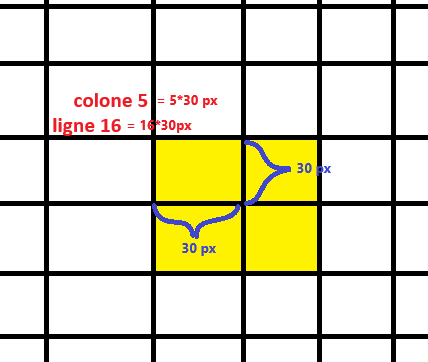
\includegraphics[scale=0.5]{ex_mino.png}
\caption{\label{dessin} Schéma représentatif d'un mino dans le plateau}
\end{figure}
\newpage
Le schéma ci-dessus prend en exemple le mino à la ligne 16 et à la conne 5.\\
On comprend d'après le schéma que le premier pixel de la ligne l est égale à 30xl, respectivement pour la colonne c nous avons 30xc. Donc nous avons la coordonnée supérieure gauche du mino dans la matrice et le buffer en ligne l et colonne c. Cependant il faudra dessiner autant de point qu'il y à de pixel dans le mino et le mino est de dimension 30x30. C'est pour cela donc que nous ajoutons "j" à la coordonné colonne et "i" à la coordonnée de ligne afin de parcourir tous les pixels du mino. 
\\\\La description plus détaillée sur l'affectation, l'utilisation et le calcule de la couleur, et la fonctionnement des boucles for se trouve au label suivant : \ref{todo2}

\section{tetris.c}
\label{tetris.c}
Le fichier tetris.c est le fichier de lequel il y a le plus de fonction. Certaines étaient déjà données par l’énoncé du projet, d'autre n'étaient pas directement visible, car elles n'étaient pas données directement comme consigne, mais elles étaient utilisées dans le programme et certaines devaient être imaginées pour faire fonctionner le programme correctement. Nous pensons que ce fichier était le plus accessible, car il ne nécessitait pas l'apprentissage d'un concept nouveau contrairement au fichier game.c \ref{game.c}, qui nécessitait de comprendre la bibliothèque SDL. De plus ce fichier permet de suivre les "états" du jeux et d'utiliser ces "états", qui changerons en fonction du temps et des actions du joueur. Ces "états" sont les différents pointeurs de la structure Tetris \ref{tetris.h}, qui sont beaucoup utilisés.
\\ le seul fichier inclue dans tetris.c est tetris.h, car tout le nécessaire y est :
\begin{itemize}
    \item La structure Tetris.
    \item Les types de tetrimino enuméré par Type.
    \item Les bibliothèques nécessaires.
    \item La déclaration des fonctions.
\end{itemize}
\begin{lstlisting}
#include "tetris.h"
\end{lstlisting}

\subsection{Initialisation du tableau tetrimino et du tableau de vitesse}
\label{tetrimino}
Pour travailler sur notre jeux il était essentielle de pouvoir représenter les différents tetrimino en fonction de type (O, I, J, L, S, Z, T) et de leurs rotations (rotation 0, rotation 1, rotation 2, rotation 3). Pour cela il a fallu initialiser " char tetriminos[7][4][5][5] ". Nous avons eu du mal à écrire ce tableau. A l'origine nous voulions le faire à l'aide de boucle for, et nous voulions le remplir par "rien" pour les cases vides et "mino" pour les cases remplies, ors bien évidemment, cela ne peut pas fonctionner car "rien" et "mino" ne sont pas des char mais des chaînes de caractères. Cependant nous avons pensé que le problème venait de la boucle for, car nous avions lu
sur un forum qu'il fallait décrire un tableau lors de son initialisation, cependant cela n'était pas le cas pour les boucles for. Nous avons donc tenté de remplir le tableau directement, mais encore une fois l'erreur persistait. C'est alors quand lisant plus précisément l'erreur et en taper l'erreur sur \href{https://openclassrooms.com/forum/sujet/message-d-erreur-29}{internet}, nous avons fini par comprendre que le problème venait du contenu du tableau et non de sa construction. Nous avons donc gardé la construction lors de l'initialisation, et cette fois le contenu est devenu '1' pour les cases remplies et '0' pour les cases vide. Pour la construction du tableau multidimensionnel nous nous somme aider du site \href{https://zestedesavoir.com/tutoriels/755/le-langage-c-1/1043_aggregats-memoire-et-fichiers/4281_les-tableaux/#3-14094_les-tableaux-multidimensionnels}{zestedesavoir}.
\\Le code de construction est le suivant :
\begin{lstlisting}
char tetriminos[7][4][5][5]={
  {/*Tetrimino I*/
    {/*Rotation 0 */
      {'0','0','0','0','0'},
      {'0','0','0','0','0'},
      {'0','1','1','1','1'},
      {'0','0','0','0','0'},
      {'0','0','0','0','0'}
    },
    {/*Rotation 1*/
      {'0','0','0','0','0'},
      {'0','0','1','0','0'},
      {'0','0','1','0','0'},
      {'0','0','1','0','0'},
      {'0','0','1','0','0'}
    },
    {/*Rotation 2*/
      {'0','0','0','0','0'},
      {'0','0','0','0','0'},
      {'1','1','1','1','0'},
      {'0','0','0','0','0'},
      {'0','0','0','0','0'}
    },
    {/*Rotation 3*/
      {'0','0','1','0','0'},
      {'0','0','1','0','0'},
      {'0','0','1','0','0'},
      {'0','0','1','0','0'},
      {'0','0','0','0','0'}
    }
  },
  {/*Tetrimino J*/
    {/*Rotation 0 */
      {'0','0','0','0','0'},
      {'0','1','0','0','0'},
      {'0','1','1','1','0'},
      {'0','0','0','0','0'},
      {'0','0','0','0','0'}
    },
    {/*Rotation 1*/
      {'0','0','0','0','0'},
      {'0','0','1','1','0'},
      {'0','0','1','0','0'},
      {'0','0','1','0','0'},
      {'0','0','0','0','0'}
    },
    {/*Rotation 2*/
      {'0','0','0','0','0'},
      {'0','0','0','0','0'},
      {'0','1','1','1','0'},
      {'0','0','0','1','0'},
      {'0','0','0','0','0'}
    },
    {/*Rotation 3*/
      {'0','0','0','0','0'},
      {'0','0','1','0','0'},
      {'0','0','1','0','0'},
      {'0','1','1','0','0'},
      {'0','0','0','0','0'}
    }
  },
  {/*Tetrimino L*/
    {/*Rotation 0*/
      {'0','0','0','0','0'},
      {'0','0','0','1','0'},
      {'0','1','1','1','0'},
      {'0','0','0','0','0'},
      {'0','0','0','0','0'}
    },
    {/*Rotation 1 */
      {'0','0','0','0','0'},
      {'0','0','1','0','0'},
      {'0','0','1','0','0'},
      {'0','0','1','1','0'},
      {'0','0','0','0','0'}
    },
    {/*rotation 2 */
      {'0','0','0','0','0'},
      {'0','0','0','0','0'},
      {'0','1','1','1','0'},
      {'0','1','0','0','0'},
      {'0','0','0','0','0'}
    },
    {/* Rotation 3 */
      {'0','0','0','0','0'},
      {'0','1','1','0','0'},
      {'0','0','1','0','0'},
      {'0','0','1','0','0'},
      {'0','0','0','0','0'}
    }
  },
  {/*Tetrimino O */
    {/* Rotation 0 */
      {'0','0','0','0','0'},
      {'0','0','0','0','0'},
      {'0','0','1','1','0'},
      {'0','0','1','1','0'},
      {'0','0','0','0','0'}
    },
    {/*Rotation 1 */
      {'0','0','0','0','0'},
      {'0','0','0','0','0'},
      {'0','0','1','1','0'},
      {'0','0','1','1','0'},
      {'0','0','0','0','0'}
    },
    {/*Rotation 2 */
      {'0','0','0','0','0'},
      {'0','0','0','0','0'},
      {'0','0','1','1','0'},
      {'0','0','1','1','0'},
      {'0','0','0','0','0'}
    },
    {/*Rotation 3 */
      {'0','0','0','0','0'},
      {'0','0','0','0','0'},
      {'0','0','1','1','0'},
      {'0','0','1','1','0'},
      {'0','0','0','0','0'}
    },
  },
  {/* Tetrimino S */
    {/* Rotation 0*/
      {'0','0','0','0','0'},
      {'0','0','1','1','0'},
      {'0','1','1','0','0'},
      {'0','0','0','0','0'},
      {'0','0','0','0','0'}
    },
    {/* Rotation 1*/
      {'0','0','0','0','0'},
      {'0','0','1','0','0'},
      {'0','0','1','1','0'},
      {'0','0','0','1','0'},
      {'0','0','0','0','0'}
    },
    {/*Rotation 2*/
      {'0','0','0','0','0'},
      {'0','0','0','0','0'},
      {'0','0','1','1','0'},
      {'0','1','1','0','0'},
      {'0','0','0','0','0'}
    },
    {/*Rotation 3 */
      {'0','0','0','0','0'},
      {'0','1','0','0','0'},
      {'0','1','1','0','0'},
      {'0','0','1','0','0'},
      {'0','0','0','0','0'}
    }
  },
  {/*Tetrimino T */
    {/* Rotation 0 */
      {'0','0','0','0','0'},
      {'0','0','1','0','0'},
      {'0','1','1','1','0'},
      {'0','0','0','0','0'},
      {'0','0','0','0','0'}
    },
    {/* Rotation 1 */
      {'0','0','0','0','0'},
      {'0','0','1','0','0'},
      {'0','0','1','1','0'},
      {'0','0','1','0','0'},
      {'0','0','0','0','0'}
    },
    {/*Rotation 2 */
      {'0','0','0','0','0'},
      {'0','0','0','0','0'},
      {'0','1','1','1','0'},
      {'0','0','1','0','0'},
      {'0','0','0','0','0'}
    },
    {/*Rotation 3 */
      {'0','0','0','0','0'},
      {'0','0','1','0','0'},
      {'0','1','1','0','0'},
      {'0','0','1','0','0'},
      {'0','0','0','0','0'}
    }
  },
  {/* Tetrimino Z */
    {/* Rotation 0 */
      {'0','0','0','0','0'},
      {'0','1','1','0','0'},
      {'0','0','1','1','0'},
      {'0','0','0','0','0'},
      {'0','0','0','0','0'}
    },
    {/*Rotation 1 */
      {'0','0','0','0','0'},
      {'0','0','0','1','0'},
      {'0','0','1','1','0'},
      {'0','0','1','0','0'},
      {'0','0','0','0','0'}
    },
    {/* Rotation 2 */
      {'0','0','0','0','0'},
      {'0','0','0','0','0'},
      {'0','1','1','0','0'},
      {'0','0','1','1','0'},
      {'0','0','0','0','0'}
    },
    {/* Rotation 3 */
      {'0','0','0','0','0'},
      {'0','0','1','0','0'},
      {'0','1','1','0','0'},
      {'0','1','0','0','0'},
      {'0','0','0','0','0'}
    }
  }
};
\end{lstlisting}
Pour correctement construire le tableau il fallait suivre l'ordre des types du tetrimino imposé par Type, l'ordre est donc le suivant : I, J, L, O, S, T, Z. Ensuite il fallait respecter l'ordre de rotation horaire de 90°, on a donc : rotation 0 = 0°, rotation 1 = 90°, rotation 2 = 180°, rotation 3 = 270°. Les deux dernières valeurs du tableau sont les emplacements des minos pour chaque tétrimino. Pour les emplacements vides nous avons décidé de les remplir par '0', et '1' pour les emplacements contenant un mino. Nous savions qu'il était possible d'utiliser la valeur 1 et 0 mais non avons préférer rester sur des char. Le contenu est donc le "dessin" en '1' et '0' de chaque tetrimino et de chaque rotation dans un tableau 5x5.
\newpage
Par exemple le tetrimino Z à la rotation 1:
\begin{lstlisting}
    ...
    ...
    },
    {
      {'0','0','0','0','0'},
      {'0','0','0','1','0'},
      {'0','0','1','1','0'},
      {'0','0','1','0','0'},
      {'0','0','0','0','0'}
    },
    {...
    ...
    ...
\end{lstlisting}
\begin{figure}[ht]
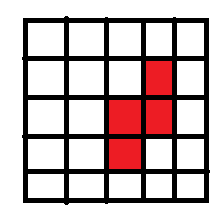
\includegraphics[scale=1]{dessin4.png}
\caption{\label{dessin1} Schéma représentatif du tetrimino Z en rotation 1}
\end{figure}
Pour le tableau de vitesse nous avons préféré le remplir directement par les valeurs approchées de chaque vitesse en fonction du niveau afin de faciliter les calcules du programme, cela permettra de rendre le jeu plus efficace. Le code est le suivant :
\label{speed}
\begin{lstlisting}
float tab2[15]={1.0,0.793,0.618,0.473,0.355,0.262,0.190,0.135,0.094,0.064,0.043,0.028,0.0018,0.011,0.007};
\end{lstlisting}
Nous aurions pu aussi faire le code suivant :
\begin{lstlisting}
float tab2[15];

for(i=1;i<=15;i++)
  {
    tab2[i]=pow(0.8-((i-1)*0.007),i-1);
  }
\end{lstlisting}
Mais comme mentionné plus haut, pour des raisons techniques, nous ne l'avons pas fait.

\subsection{Les fonctions aléatoires}
\label{alea}
\label{init_alea}
L'utilisation de fonctions aléatoires était nécessaire pour le bon fonctionnement du jeu, car pour choisir le premier tétrimino du jeu et le tétrimino suivant il fallait une fonction pour le faire. Plus précisément une fonction qui choisit un nombre entre 0 et 6, valeur égale au type de tetrimino associé. Pour l'implémentation des ces fonctions nous nous sommes aidés d'un forum sur \href{https://openclassrooms.com/forum/sujet/generateur-de-nombre-aleatoire-entre-1-et-9}{openclassrooms} et du site \href{https://nicolasj.developpez.com/articles/libc/hasard/}{developpez} pour mieux comprendre leurs utilisations et comment les coder.
La fonction aléatoire à eu deux formes, la première était celle-ci :
\begin{lstlisting}
int alea()
{
//Initialisation d'un générateur d'aléatoire
  srand(time(NULL));
  return rand()%7;;
}
\end{lstlisting}
Nous avons donc initialisé un générateur de nombre aléatoire pour que la fonction renvoie un nombre aléatoire entre 0 et 6.
\\ A la ligne \textcolor{gris}{4} la fonction srand() initialise un générateur de nombre aléatoire basé sur l'heure.
\\Ligne \textcolor{gris}{5} on retourne un nombre aléatoire compris entre 0 et 7 grâce au modulo 7.
\\\\
Cette fonction fonctionnait très bien initialement, mais nous pouvions constater lors de l'utilisation du jeu que certains tetriminos se répétaient. Cela était dû au générateur aléatoire qui, étant basé sur l'heure, si la seconde entre deux tétriminos était la même, les tétriminos seraient les mêmes, rendant le jeu plus répétitif. Nous avons donc décidé de changer le code pour celui-ci:
\begin{lstlisting}
//Initialisation d'un générateur d'aléatoire
void init_alea()
{
  srand(time(NULL));
}

//Renvoie un nombre aléatoire entre 0 et 6.
int alea()
{
  return rand()%7;;
}
\end{lstlisting}
Ainsi un unique générateur aléatoire est initialisé au début du jeu avec init\_alea() et alea() renverra une valeur "réellement" aléatoire.

\subsection{tetris\_new()}
\label{tetris_new}
Cette fonction n'est utilisée qu'une seule fois dans la fonction game\_new() \ref{game_new}, car elle permet d'initialiser un nouveau setup Tetris, elle ne sera donc pas utilisée ailleurs.
\\Le code est le suivant :
\begin{lstlisting}
Tetris *tetris_new()
{
  Tetris *t;
  int i;
  int j;

  //Allocation dans la mémoire
  t=malloc(sizeof(Tetris));
  if(t==NULL)
    return NULL;

  //Remplissage du buffer et de la matrice de '0'.
  for (i=0;i<20;i++)
    {
      for(j=0;j<10;j++)
	{
	  t->matrix[i][j]='0';
	  t->buffer[i][j]='0';
	}
    }

  //Choix d'un premier type aléatoire
  t->current_type=alea();

  //Positionnement sur la premiere ligne en fonction du type
  if(t->current_type==0||t->current_type==3)
    {
      t->current_line=0;
    }
  else
    {
      t->current_line=1;
    }

  //Posistionnement sur le colonne 4 pour centrer le tetrimino
  t->current_column=4;


  t->current_rotation=0;

  t->next_type=alea();

  t->level=1;
  t->score=0;
  t->nbr_lines=0;

  for(i=0;i<15;i++)
    {
      //Remplir le tableau par des valeurs prédéfinies est plus intéressant que de faire les calcules pour des questions de vitesse.
      t->drop_speed[i]=tab2[i];
    }
  return t;
}
\end{lstlisting}
Premièrement il faut initialiser les éléments nécessaires. Le pointeur t de type Tetris et les entiers i et j pour faire des boucles for.
\\\\
Ensuite de la ligne \textcolor{gris}{8} à \textcolor{gris}{9} on alloue de la mémoire et on teste si l'allocation c'est bien passée.
\\\\
Ensuite de la ligne \textcolor{gris}{13} à \textcolor{gris}{20} on utilise une double boucle for pour remplir les pointeurs du buffer et de la matrice de t de '0' élément considérer nul. Cela permet de bien avoir un nouveau jeu à la ligne \textcolor{gris}{23}.
\\\\
Puis nous utilisons la fonction alea() pour choisir un type pour le premiers tetrimino du jeu.
\\\\
Pour le pointeur de ligne et de colonne actuelle de t, la valeur de la colonne sera 4 et le ligne dépendra du pointeur de tetrimino actuel. Car si le tetrimino est O ou I, en rotation 0 il y a assez de place pour les mettre sur la ligne 0 du buffer, sinon la ligne sera 1. Cela a été défini par le tableau tetrimino \ref{tetrimino}. Le pointeur de rotation actuel de t est 0 et le pointeur du prochain tétrimino de t est une valeur encore aléatoire entre 0 et 6.
\\\\ On pointe ensuite le score à 0, le niveau à 1 et le nombre de ligne détruite à 0 et on remplit le pointeur drop\_speed de t par les valeurs du tableau de vitesse \ref{speed}.
\\Enfin on retourne t.

\subsection{tetris\_del()}
\label{tetris_del}

\begin{lstlisting}
void tetris_del(Tetris *tet)
{
  free(tet);
}
\end{lstlisting}
La fonction est très courte et nécessite qu'une seul ligne, car il n'y a qu'une seule allocation de mémoire nécessaire lors de la création d'un nouveau Tetris. Donc utiliser la fonction free() pour libérer la mémoire allouée par tet est suffisant.

\subsection{tetris\_reset()}
\label{tetris_reset}
Cette fonction à pour but de relancer un nouveau tetrimino une fois que le tetrimino actuel ne peut plus descendre. Elle prend en argument un pointer appelé tet de type Tetris.
\begin{lstlisting}
void tetris_reset(Tetris *tet)
{
  int i;
  int j;

  tet->current_type=tet->next_type;
  tet->next_type=alea();
  tet->current_column=4;
  tet->current_rotation=0;

  //Remise du buffer à '0'
  for (i=0;i<20;i++)
    {
      for(j=0;j<10;j++)
	{
	  tet->buffer[i][j]='0';
	}
    }

  //Positionnement du tetrimino dans le buffer en fonction de son type
  if(tet->current_type==0||tet->current_type==3)
    {
      tet->current_line=0;
      for(i=2;i<=4;i++)
	{
	  for(j=0;j<=4;j++)
	    {
	      tet->buffer[i-2][j+2]=tetriminos[tet->current_type][tet->current_rotation][i][j];
	    }
	}
    }
  else
    {
      tet->current_line=1;
      for(i=1;i<=4;i++)
	{
	  for(j=0;j<=4;j++)
	    {
	      tet->buffer[i-1][j+2]=tetriminos[tet->current_type][tet->current_rotation][i][j];
	    }
	}
    }
}
\end{lstlisting}
Le code commence donc par initialiser deux entiers pour faire des doubles boucles for (ligne \textcolor{gris}{3} et \textcolor{gris}{4})
\\\\
Par le suite nous devons implémenter le nouveau tetrimino, pour cela nous commençons par faire pointer le type actuel vers le pointeur du prochain type de tet. Cela à pour effet de faire passer le prochain type en type actuel (ligne \textcolor{gris}{6}).
\\\\
Après il faut définir un nouveau type pour le pointeur du prochain type avec la fonction alea() (ligne \textcolor{gris}{7}).
\\\\
Il faudra aussi remettre le pointeur à la colonne 4 et la rotation à 0 pour centrer le tetrimino dans sa position initiale (ligne \textcolor{gris}{8} et \textcolor{gris}{9}).
\\\\
Puis on remet le pointeur du buffer à '0' avec une double boucle for (ligne \textcolor{gris}{12} à \textcolor{gris}{18})
\\\\
Enfin, il faut mettre le nouveau tetrimino dans le buffer à la ligne correspondante en fonction du type. 
\\Donc si le type actuel du tetrimino est O ou I (0 ou 3) alors la ligne actuelle sera 0 sinon la ligne sera 1. Dans ces deux conditions on y ajoute deux boucles for la première est le suivante :
\begin{lstlisting}
for(i=2;i<=4;i++)
	{
	  for(j=0;j<=4;j++)
	    {
	      tet->buffer[i-2][j+2]=tetriminos[tet->current_type][tet->current_rotation][i][j];
	    }
	}
\end{lstlisting}
Ici nous sommes dans le cas où le tetrimino est de type O ou I. Nous commençons par une boucle for allant de 2 à 4 car les deux premières lignes du tetrimino sont vides, puis nous poursuivons une autre boucle for qui parcourt l'ensemble des colonnes. Ensuite dans ces deux boucles for on effectue la commande suivante :
\begin{equation*}
    \text{tet->buffer[i-2][j+2]=tetriminos[tet->current\_type][tet->current\_rotation][i][j];}
\end{equation*}
Cela aura pour effet de placer le tetrimino dans la partie supérieur centré du buffer.
Illustrons un exemple avec un dessin.
\begin{figure}[ht]
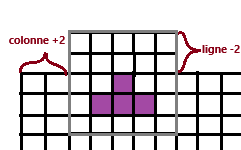
\includegraphics[scale=1]{buffer_tetrimino.png}
\caption{\label{dessin3} Schéma de tetris\_reset}
\end{figure}
On illustre avec le schéma que les valeurs i-2 et j+2, que nous avons utilisées permettent de faire correspondre la colonne et la ligne du tetrimino à sa place dans le buffer. Nous ajoutons 2 pour la colonne soustrayons 2 pour la ligne.
\\\\
Le travail est le même pour les autres types de tetrimino à la différence que nous faisons une première boucle pour les lignes allant de 1 à 4, car uniquement la première ligne sera vide.

\newpage
\subsection{teris\_can\_go\_left()}
Elle prend en argument un pointeur de type Tetris et renvoie 1 si le tetrimino peut aller à gauche et 0 sinon. Cette fonction est utilisée pour vérifier si l'évènement "aller à gauche" est possible \ref{left}. Cette fonction ainsi que les autres fonctions tetris\_can étaient au début difficile à comprendre car il fallait trouver une méthode pour que les minos associés au tetrimino soient reconnus au bonne endroit dans le buffer, afin de faire les testes. Cependant une fois la méthode trouvée pour une fonction, il ne fallait plus que la répéter pour le reste. Il s'agit aussi des fonctions pour lesquelles nous avons rencontré le plus de bug, notamment beaucoup de dépassement de limite. Ces bug étaient principalement dû à des coquilles dans le code.
\label{tetris_can_go_left}
\begin{lstlisting}
int tetris_can_go_left(Tetris *tet)
{
  int i;
  int j;

  for(i=0;i<5;i++)
    {
      for(j=0;j<5;j++)
	{
	  //On cherche les case remplies par tetrimino
	  if(tetriminos[tet->current_type][tet->current_rotation][i][j] == '1')
	    {
	      //ici on teste si la colonne à gauche du mino est toujours dans le tableau et on teste si la case à gauche du mino est remplie ou non
	      //le calcule "current_column + j - 2" nous permet d'avoir la position du mino
	      if(tet->current_column + j-3 <0 || tet->matrix[tet->current_line + i -2][tet->current_column + j-3] == '1')
		return 0;
	    }
	}
    }
  return 1;
}
\end{lstlisting}
Les commentaires expliquent quelque peu le code cependant penchons nous sur la raison de cette méthode.
\\Nous commençons par faire une double boucle for avec i et j allant de 0 à 5 pour parcourir tout le tetrimino et tester si une case du tetrimino est égale à '1', donc pour vérifier si il y à un mino à cet endroit du tableau. Une fois l'emplacement localisé il faut refaire un teste pour vérifier si la case de la matrice située à gauche du mino est vide ou non (dans la matrice).
\\Pour cela il faut accéder à la valeur de la ligne actuelle et la colonne actuelle dans le buffer du mino correspondant. On utilise alors les valeurs suivantes:
\begin{equation*}
\begin{split}
    \text{tet->current\_column + j - 2}
    \\\\
    \text{tet->current\_line + i - 2}
\end{split}
\end{equation*}
Cette méthode fonctionne quelque soit le tetrimino.
\begin{figure}[ht]
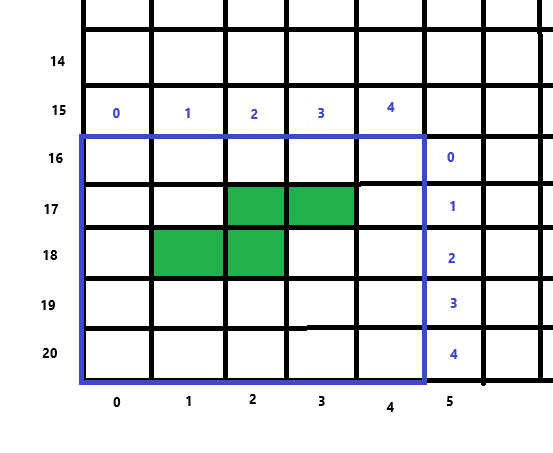
\includegraphics[scale=0.5]{dessin5.png}
\caption{\label{dessin4} Schéma d'un tetrimino dans le buffer}
\end{figure}
D'après le dessin si nous faisons tous les calcules en fonction de la ligne et de la colonne dans le tableau tetrimino, qu'on soustrait par 2 nous obtenons les bons résultats.
\\Inutile de tester pour les colonnes.
Pour les lignes nous avons bien :
\begin{equation*}
    \begin{split}
        \text{tet->current\_line + 0 - 2}=18+0-2=16
        \\
        \text{tet->current\_line + 1 - 2}=18+1-2=17
        \\
        \text{tet->current\_line + 2 - 2}=18+2-2=18
        \\
        \text{tet->current\_line + 3 - 2}=18+3-2=19
        \\
        \text{tet->current\_line + 4 - 2}=18+4-2=20
    \end{split}
\end{equation*}
Une fois qu'on a accédé à la position dans le buffer on vérifie si dans la position à la même ligne, une colonne à gauche il y à un mino ou si nous nous trouvons à l'extérieur du plateau. Pour cela on fait un teste sur tet->current\_column + j - 2 - 1, dans la matrice et dans les valeurs du tableau.
\\Donc si la cases à gauche du mino est remplie dans la matrice ou que l'emplacement à gauche du mino est un emplacement en dehors du terrain (emplacement inférieur à 0), alors on retourne 0, sinon on retourne 1.
\\Il est intéressant de préciser qu'il n'y aura pas de conflit si le mino sélectionné dans le buffer est un mino positionné à droite d'un autre mino dans le buffer, car la comparaison se fait entre le buffer et la matrice, ce qui implique que les minos sélectionnés dans le buffer ne sont pas dans la matrice.

\subsection{tetris\_can\_go\_right()}
\label{tetris_can_go_right}
Elle prend en argument un pointeur de type Tetris et renvoie 1 si le tetrimino peut aller à droite et 0 sinon. Elle est utilisée pour vérifier si l'évènement, pour le déplacement à droite, est possible \ref{right}.
La fonction teris\_can\_go\_right() est quasiment identique à la fonction tetris\_can\_go\_left(), à la différence que nous ne travaillons plus sur le colonne à gauche du mino, mais sur la colonne à droite. Voici le code :
\begin{lstlisting}
int tetris_can_go_right(Tetris *tet)
{
  int i;
  int j;

  for(i=0;i<5;i++)
    {
      for(j=0;j<5;j++)
	{
	  if(tetriminos[tet->current_type][tet->current_rotation][i][j] == '1')
	    {
	      if((tet->current_column + j - 1 >=10) || (tet->matrix[tet->current_line +i -2][tet->current_column + j -1] == '1'))
		return 0;
	    }
	}
    }
  return 1;
}
\end{lstlisting}
Donc la différence entre tetris\_can\_go\_right() et tetris\_can\_go\_left() est dans la dernière condition. Cette fois nous voulons vérifier si la case dans la colonne de droite est remplie ou non et si la colonne de droite est toujours dans le plateau du jeux. Donc nous vérifions de la même façons que dans tetris\_can\_go\_left() cependant nous le vérifions à la colonne  tet->current\_column + j - 2 + 1. De plus pour être sûr que l'emplacement est bien dans le terrain de jeu il faut que cette valeur soit cette fois inférieur strictement à 10.

\subsection{tetris\_can\_rotate\_h()}
\label{tetris_can_rotate_h}
Elle prend en argument un pointeur de type Tetris et renvoie 1 si le tetrimino peut tourner dans le sens horaire et 0 sinon.
La fonction est utilisée pour vérifier si nous pouvons actionner l'évènement rotation horaire \ref{rotate_h}.
Cette fonction ressemble également au précédente et suit un même principe qui est de vérifier si les tetriminos dans la matrice gène l'évènement.
\begin{lstlisting}
for(i=0;i<5;i++)
    {
      for(j=0;j<5;j++)
	{
	  //Teste spécifique pour revenir à la rotation 0
	  if(tet->current_rotation + 1 == 4)
	    {
	      if(tetriminos[tet->current_type][0][i][j]=='1')
		{
		  //On teste si des minos bloquent la rotation, ou si le tetrimino dépasse les limites du jeux.
		  if(tet->matrix[tet->current_line +i -2][tet->current_column + j -2]=='1' ||tet->current_column +j-2 < 0 || tet->current_column+j-2>=10 || tet->current_line +i-2 >=20 ||tet->current_line +i-2 <0 )
		    return 0;
		}
	    }
	
	      
	  else if(tetriminos[tet->current_type][tet->current_rotation+1][i][j]=='1')
	    {
	      if(tet->matrix[tet->current_line +i -2][tet->current_column + j -2]=='1' ||tet->current_column +j-2 < 0 || tet->current_column+j-2>=10 || tet->current_line +i-2 >=20 ||tet->current_line +i-2 <0 )
		return 0;
	    }
	}
    }
  return 1;
}
\end{lstlisting}
Pour commencer nous faisons donc une double boucle for, puis il faut faire un teste sur le pointeur de rotation actuelle pour éviter un bug. Si nous ne faisons pas ce teste nous obtenons ce bug :
\begin{figure}[ht]
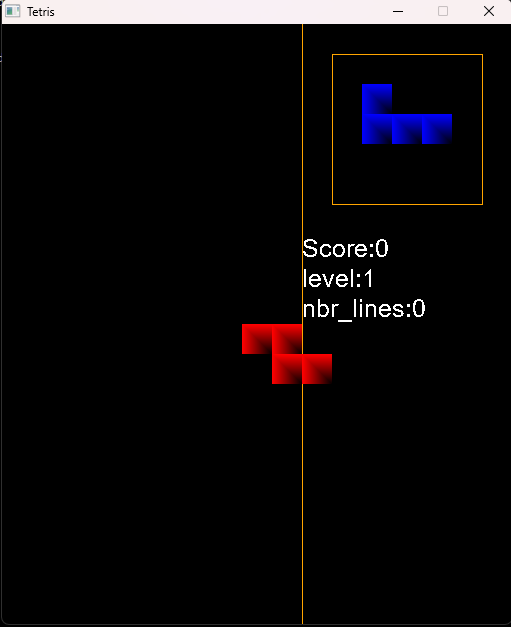
\includegraphics[scale=0.5]{CE1.png}
\caption{\label{bug1} Bug du Tetris}
\end{figure}
Donc à l'issue de ce teste pour rester dans les rotations possibles du tetrimino, nous vérifions si les emplacements dans la matrice de la rotation suivante du tetrimino sont libres ou non et également que le tetrimino reste dans les bordures du terrain. Pour cela nous commençons par identifier les lignes et les colonnes où seront potentiellement placés les minos puis on fait le teste suivant :
\begin{equation*}
\begin{split}
    \text{ tet->matrix[tet->current\_line + i -2][tet->current\_column + j -2]== ’1 ’ || tet->
current\_column +j -2 < 0}
\\
\text{|| tet->current\_column +j -2 >=10 || tet->current\_line +i -2 >=20 ||
tet->current\_line +i -2 <0 }
\end{split}
\end{equation*}
Si le teste est vrai on retourne 0 sinon on retour 1. Dans le cas ou l'incrémentation de la rotation est égale à 4 on remplace tet->current\_rotation par 0 pour que le programme fonctionne correctement.

\subsection{tetris\_can\_rotate\_ah}
\label{tetris_can_rotate_ah}
Elle prend en argument un pointeur de type Tetris et renvoie 1 si le tetrimino peut tourner dans le sens anti-horaire et 0 sinon. Elle est utilisée pour effectuer l'évènement de rotation anti-horaire \ref{rotate_ah}. Elle est quasiment la même que la fonction précédente hormis que dans celle-ci le premier teste sur la rotation actuel est en fonction de la décrémentation de celui-ci, car si la rotation actuelle -1 est égale à -1, cela veut dire que nous avons effectué une rotation complète donc la rotation actuelle doit être égale à 3. Le code est le suivant :
\begin{lstlisting}
int tetris_can_rotate_ah(Tetris *tet)
{
  int i;
  int j;

  for(i=0;i<5;i++)
    {
      for(j=0;j<5;j++)
	{
	  if(tet->current_rotation - 1 == -1)
	    {
	      if(tetriminos[tet->current_type][3][i][j]=='1')
		{
		  if(tet->matrix[tet->current_line +i -2][tet->current_column + j -2]=='1' ||tet->current_column +j-2 < 0 || tet->current_column+j-2>=10 || tet->current_line +i-2 >=20||tet->current_line +i-2 <0 )
		    return 0;
		}
	    }
	      
	  if(tetriminos[tet->current_type][tet->current_rotation-1][i][j]=='1')
	    {
	      if(tet->matrix[tet->current_line +i -2][tet->current_column + j -2]=='1' ||tet->current_column +j-2 < 0 || tet->current_column+j-2>=10 || tet->current_line +i-2 >=20||tet->current_line +i-2 <0 )
		return 0;
	    }
	}
    }
  return 1;
}
\end{lstlisting}
Donc cette fois-ci nous travaillons sur la rotation précédente et non la rotation suivante, d'où les testes pour tet->current\_rotation-1.

\subsection{tetris\_can\_go\_down()}
\label{tetris_can_go_down}
Elle prend en argument un pointeur de type Tetris et renvoie 1 si le tetrimino peut descendre et 0 sinon. Elle est utilisée pour l'évènement "descendre une case" \ref{down} et l'évènement "descendre tout en bas" \ref{down_down} et dans la fonction game\_run \ref{if_down}. Elle est quasiment identique à la fonction tetris\_can\_go\_right(), sauf que cette fois-ci il sera question de vérifier la ligne d'en-dessous et de vérifier si la ligne suivant est inférieur à 20. Voici le code:
\begin{lstlisting}
int tetris_can_go_down(Tetris *tet)
{
  int i;
  int j;

  for(i=0;i<5;i++)
    {
      for(j=0;j<5;j++)
	{
	  if(tetriminos[tet->current_type][tet->current_rotation][i][j]=='1')
	    {
	      //On teste si un mino est en dessous du tetrimino ou si le tetrimino dépasse le terrain.
	      if((tet->current_line + i -1 >= 20)  || (tet->matrix[tet->current_line +i -1][tet->current_column + j -2]=='1'))
		return 0;
	    }
	}
    }
  return 1;
}
\end{lstlisting}
Comme les précédentes fonction il sera question d'identifier les cases du tetrimino qui sont remplies avec une double boucle for et un teste en fonction du pointeur de type actuel, du pointeur de rotation actuel et la colonne j et la ligne i en question. Ensuite pour vérifier si le tetrimino peut descendre on utilise la valeur de ligne suivante :
\begin{equation*}
    \text{tet->current\_line + i -2 + 1}
\end{equation*}
Avec cela, comme dans les précédentes fonctions on vérifie la contenance de la case en-dessous et on vérifie si l'indice de la ligne du dessous est supérieur à 20. Si le tetrimino dépasse le terrain ou si il y a un mino en-dessous alors on retourne 0, sinon 1.

\subsection{tetris\_get\_drop\_speed()}
\label{tetris_get_drop_speed}
Cette fonction permet d'obtenir la vitesse actuelle du jeux en fonction du niveau, elle est utilisé dans le fonction game\_run(). Son code est le suivant :
\begin{lstlisting}
double tetris_get_drop_speed(Tetris *tet)
{
  return pow(0.8-((tet->level -1)*0.007),tet->level -1);
}
\end{lstlisting}
Elle prend donc en argument un pointeur de type Tetris et renvoie la vitesse en fonction du pointeur sur le niveau. On utilise aussi la fonction pow() provenant de la bibliothèque math.h.

\subsection{tetris\_matrix\_update()}
\label{tetris_matrix_update}
Elle fait partie d'une des fonctions que nous avons dû imaginer pour que le programme fonction correctement, car initialement nous voulions mettre à jour directement la matrice dans la fonction game\_run(), mais cela causait des problèmes de compilation si nous déclarions le tableau tetrimino dans tetris.h et si nous l'incluons dans game.c. Donc il était plus judicieux de programmer une fonction dans tetric.c.
\begin{lstlisting}
void tetris_matrix_update(Tetris *tet)
{
  int i;
  int j;
  for(i=0;i<5;i++)
    {
      for(j=0;j<5;j++)
	{
	  if(tetriminos[tet->current_type][tet->current_rotation][i][j]=='1')
	    {
	      tet->matrix[tet->current_line+i-2][tet->current_column+j-2]=tetriminos[tet->current_type][tet->current_rotation][i][j];
	    }
	}
    }
}
\end{lstlisting}
Le programme est assez simple, nous parcourons le tableau tetrimino avec une double boucle for de 0 à 5, pour identifier les cases remplies, une fois cela fait nous les affectons aux pointeurs de la matrice correspondants en fonction de la colonne j et de la ligne i.

\subsection{tetris\_shift\_board()}
\label{tetris_shift_board}
Cette fonction prend en argument un pointeur de type Tetris et à pour effet de faire descendre tous les minos une fois qu'une ou plusieurs destructions de ligne ait été effectuées. Le code est le suivant :
\begin{lstlisting}
void tetris_shift_board(Tetris *tet)
{
  int i;
  int j;
  int k;
  int count;
 
for(i=0;i<20;i++)
  {
    count=0;
    for(j=0;j<10;j++)
	{
	  if(tet->matrix[i][j]=='1')
	    {
	      count+=1;
	    }
	}
    //Teste si une ligne est complis
      if(count == 10)
	{
	  //Remplir la ligne de '0'
	  for(j=0;j<10;j++)
	    {
	      tet->matrix[i][j]='0';
	    }
	  //Parcourt le tableau de bas en haut
	  for(k=i;k>0;k--)
	    {
	      //Colonne par colonne
	      for(j=0;j<10;j++)
		{
		  //Affecte la ligne du dessus à la ligne du dessous
		  tet->matrix[k][j]=tet->matrix[k-1][j];
		}
	    }
	  //Necessaire dans le cas ou la premiers ligne est remplie de mino.
	  //Car la ligne 0 n'est pas affécté à la ligne 1;
	  for(j=0;j<10;j++)
	    {
	      tet->matrix[0][j]='0';
	    }
	}
    }
}
\end{lstlisting}
Pour le bon fonctionnement du code il nous faut 3 entiers pour les boucles et une variable de contage que nous initialisons.
\\Initialement nous ne voulions pas parcourir le tableau dans sont intégralité mais plutôt se restreindre au ligne dans les quelles le tetrimino se situe et par la suite faire un travail sur le nombre de ligne à éliminées et leurs emplacement, etc. Cependant c'est une méthode compliqué une fois arriver à la descente des minos. Nous avons alors préféré opter pour un parcours complet du tableau qui facilitera la descente des minos.
\\\\
Donc nous commençons par une boucle for sur i allant de 0 à 19 pour parcourir toutes les lignes. Nous affectons ensuite à notre compteur la valeur de 0, puis de la ligne \textcolor{gris}{11} à la ligne \textcolor{gris}{16} nous effectuons notre comptage pour vérifier si la ligne est remplie. Il suffit d'incrémenter de 1 count et si à la sortie de la boucle, count est égal à 10 alors la ligne est remplie.
\\Donc si cette condition est vérifiée on commence d'abord par remplir la ligne de '0' (ligne \textcolor{gris}{22} à \textcolor{gris}{25}).
\\\\
Puis toujours en respectant la condition de comptage, nous effectuons une double boucle for, cette fois pour faire descendre les minos. La première boucle sera alors une boucle qui remontera les lignes à partir de la ligne remplie, donc k est affectée à i, et tant que k est supérieure à 0, nous décrémentons k. Il faut préciser que nous devons nous arrêter à 1 pour éviter de sortir du tableau. La seconde boucle va parcourir toutes les colonnes et la ligne \textcolor{gris}{33} aura pour effet de faire descendre le mino au-dessus de la ligne k.
\\\\Pour finir nous faisons une dernière boucle for dans la première boucle for i, afin de remplir la première ligne de '0', au cas où si la ligne contenait des minos.

\section{game.c}
\label{game.c}
Nous allons maintenant voir le contenue du fichier game.c, en présentant chaque fonction de ce fichier. Comme déjà mentionné le site \href{https://zestedesavoir.com/tutoriels/1014/utiliser-la-sdl-en-langage-c/}{zestedesavoir} a été essentielle pour la réussite du programme. Grâce au contenue du site, nous avons pu comprendre comment fonctionnent les différentes commandes de la SDL et en apprendre de nouvelles pour faciliter le codage, comme la création de ligne et de rectangle. Également, le travaille de Cam dans la \href{https://www.youtube.com/watch?v=NQZNHUoba-8&t=458s}{première} et \href{https://www.youtube.com/watch?v=LS_eeI-9-pA&t=11s}{deuxième} vidéo sur l'utilisation de TTF\_font nous a permis d'obtenir des résultats important sur l'affichage.
\\Cela nous à donc permit de résoudre les problèmes du projet avec ces outils. Parfois sans succès, notamment dans la fonction mino\_display() \ref{mino_display} ou dans le TODO n°2 \ref{todo2}, mentionné plus bas, où nous avons dû rester sur des méthodes plus accessibles. Mais nous pensons que le point le plus important était sur l'utilisation des commandes permettant de créer et de fermer des fenêtres ou des rendus, car si cette partie du travaille n'était pas correctement effectuée, il n'y aurait pas pu y avoir d'affichage.
\subsection{Inclusion de fichier d'en-tête et déclaration de variable global}
\label{debut_game}
\begin{lstlisting}
#include "game.h"
#include "mino.h"

static int update =1;
\end{lstlisting}
Nous incluons game.h pour pouvoir utiliser les bibliothèques nécessaires et la structure Game. Nous initialisons également update à 1 comme variable global car elle est utilisé dans deux fonctions du fichier.

\subsection{game\_board\_update()}
\label{game_board_update}
Cette fonction prend en argument un pointeur de type Game et elle renvoie un affichage dans une fenêtre. 
\\ Cette fonction a été l'une des plus longue à coder, nous n'avons pas trouvé d'autre moyens que de répéter plusieurs fois des lignes de codes très similaires. Cependant l'étude de l'utilisation de la bibliothèque SDL à aussi été d'une très grande aide pour l'écriture de cette fonction. Pour présenter la fonction nous allons la découper en quatre parties.
\begin{itemize}
    \item L'initialisation et la clôture de la fonction
    \item TODO n°1 : afficher le plateau de jeu \ref{todo1}
    \item TODO n°2 : afficher le prochain tetrimino \ref{todo2}
    \item TODO n°3 : afficher le score, le niveau et le nombre de lignes eliminées \ref{todo3}
\end{itemize}
\subsubsection{L'initialisation et la clôture de la fonction}
\begin{lstlisting}
static void game_board_update(Game *g)
{
  int i;
  int j;
  int z;

  SDL_SetRenderDrawColor(g->ren, 0x2b, 0x2a, 0x33, 0xff);
  SDL_RenderClear(g->ren);
  ...
  ...
  ...
  //Suite du programme
  ...
  ...
  ...
  SDL_RenderPresent(g->ren);

  update = 0;
}
\end{lstlisting}
Nous initialisons les variables entières i, j et z car nous allons les utiliser dans des boucles for.
\\Les lignes \textcolor{gris}{13} permettent d'afficher le rendu du du pointeur de g sur le rendu à l'écran.
\\Dans la partie suite du programme nous aurons les TODO.

\subsubsection{TODO n°1 : afficher le plateau de jeu}
\label{todo1}
\begin{lstlisting}
// Colorer le fond du plateau en noir
  SDL_Color black = {0,0,0,255};
  SDL_SetRenderDrawColor(g->ren,black.r,black.g,black.b,black.a);
  SDL_RenderClear(g->ren);

  /*Bordure du plateau de jeux*/
  SDL_Color orange = {255,165.75,0,255};
  SDL_SetRenderDrawColor(g->ren,orange.r,orange.g,orange.b,orange.a);
  SDL_RenderDrawLine(g->ren,300,600,300,0);

  //Dessiner un rectangle en haut à droite
  SDL_SetRenderDrawColor(g->ren,orange.r,orange.g,orange.b,orange.a);
  SDL_Rect r={330,30,151,151};
  SDL_RenderDrawRect(g->ren,&r);

  //Affichage des minos dans le plateau de jeux pour avoir un visuel de la matrix.
  for(i=0;i<20;i++)
    {
      for(j=0;j<10;j++)
	{
	  if(g->tet->matrix[i][j]=='1')
	    {
	      mino_display(g,g->tet->current_type,i,j);
	    }
	}
    }
    
  //Affichage du tetrimino actuelle, qui est  présent dans le buffer. 
  if(g->tet->current_type==0)
    {//Tetrimino I
      if(g->tet->current_rotation==0)
	{//Rotation 0
	  mino_display(g,g->tet->current_type,g->tet->current_line,g->tet->current_column-1);
	  mino_display(g,g->tet->current_type,g->tet->current_line,g->tet->current_column);
	  mino_display(g,g->tet->current_type,g->tet->current_line,g->tet->current_column+1);
	  mino_display(g,g->tet->current_type,g->tet->current_line,g->tet->current_column+2);
	}
      else if(g->tet->current_rotation==1)
	{//Rotation 1
	  mino_display(g,g->tet->current_type,g->tet->current_line-1,g->tet->current_column);
	  mino_display(g,g->tet->current_type,g->tet->current_line,g->tet->current_column);
	  mino_display(g,g->tet->current_type,g->tet->current_line+1,g->tet->current_column);
	  mino_display(g,g->tet->current_type,g->tet->current_line+2,g->tet->current_column);
	}
      else if(g->tet->current_rotation==2)
	{//Rotation 2
	  mino_display(g,g->tet->current_type,g->tet->current_line,g->tet->current_column+1);
	  mino_display(g,g->tet->current_type,g->tet->current_line,g->tet->current_column);
	  mino_display(g,g->tet->current_type,g->tet->current_line,g->tet->current_column-1);
	  mino_display(g,g->tet->current_type,g->tet->current_line,g->tet->current_column-2);
	}
      else if(g->tet->current_rotation==3)
	{//Rotation 3
	  mino_display(g,g->tet->current_type,g->tet->current_line+1,g->tet->current_column);
	  mino_display(g,g->tet->current_type,g->tet->current_line,g->tet->current_column);
	  mino_display(g,g->tet->current_type,g->tet->current_line-1,g->tet->current_column);
	  mino_display(g,g->tet->current_type,g->tet->current_line-2,g->tet->current_column);
	}
    }
  else if(g->tet->current_type==1)
    {//Tetrimino J
      if(g->tet->current_rotation==0)
	{//Rotation 0
	  mino_display(g,g->tet->current_type,g->tet->current_line-1,g->tet->current_column-1);
	  mino_display(g,g->tet->current_type,g->tet->current_line,g->tet->current_column-1);
	  mino_display(g,g->tet->current_type,g->tet->current_line,g->tet->current_column);
	  mino_display(g,g->tet->current_type,g->tet->current_line,g->tet->current_column+1);
	}
      else if(g->tet->current_rotation==1)
	{//Rotation 1
	  mino_display(g,g->tet->current_type,g->tet->current_line-1,g->tet->current_column);
	  mino_display(g,g->tet->current_type,g->tet->current_line-1,g->tet->current_column+1);
	  mino_display(g,g->tet->current_type,g->tet->current_line,g->tet->current_column);
	  mino_display(g,g->tet->current_type,g->tet->current_line+1,g->tet->current_column);
	}
      else if(g->tet->current_rotation==2)
	{//Rotation 2
	  mino_display(g,g->tet->current_type,g->tet->current_line,g->tet->current_column-1);
	  mino_display(g,g->tet->current_type,g->tet->current_line,g->tet->current_column+1);
	  mino_display(g,g->tet->current_type,g->tet->current_line,g->tet->current_column);
	  mino_display(g,g->tet->current_type,g->tet->current_line+1,g->tet->current_column+1);
	}
      else if(g->tet->current_rotation==3)
	{//Rotation 3
	  mino_display(g,g->tet->current_type,g->tet->current_line-1,g->tet->current_column);
	  mino_display(g,g->tet->current_type,g->tet->current_line+1,g->tet->current_column-1);
	  mino_display(g,g->tet->current_type,g->tet->current_line,g->tet->current_column);
	  mino_display(g,g->tet->current_type,g->tet->current_line+1,g->tet->current_column);
	}
    }
  else if(g->tet->current_type==2)
    {//Tetrimino L
      if (g->tet->current_rotation==0)
	{//Rotation 0
	  mino_display(g,g->tet->current_type,g->tet->current_line,g->tet->current_column-1);
	  mino_display(g,g->tet->current_type,g->tet->current_line,g->tet->current_column);
	  mino_display(g,g->tet->current_type,g->tet->current_line,g->tet->current_column+1);
	  mino_display(g,g->tet->current_type,g->tet->current_line-1,g->tet->current_column+1);
	}
      else if (g->tet->current_rotation==1)
	{//Rotation 1
	  mino_display(g,g->tet->current_type,g->tet->current_line-1,g->tet->current_column);
	  mino_display(g,g->tet->current_type,g->tet->current_line,g->tet->current_column);
	  mino_display(g,g->tet->current_type,g->tet->current_line+1,g->tet->current_column);
	  mino_display(g,g->tet->current_type,g->tet->current_line+1,g->tet->current_column+1);
	}
      else if (g->tet->current_rotation==2)
	{//Rotation 2
	  mino_display(g,g->tet->current_type,g->tet->current_line,g->tet->current_column-1);
	  mino_display(g,g->tet->current_type,g->tet->current_line,g->tet->current_column);
	  mino_display(g,g->tet->current_type,g->tet->current_line,g->tet->current_column+1);
	  mino_display(g,g->tet->current_type,g->tet->current_line+1,g->tet->current_column-1);
	}
      else if (g->tet->current_rotation==3)
	{//Rotation 3
	  mino_display(g,g->tet->current_type,g->tet->current_line-1,g->tet->current_column);
	  mino_display(g,g->tet->current_type,g->tet->current_line,g->tet->current_column);
	  mino_display(g,g->tet->current_type,g->tet->current_line+1,g->tet->current_column);
	  mino_display(g,g->tet->current_type,g->tet->current_line-1,g->tet->current_column-1);
	}
    }
  else if(g->tet->current_type==3)
    {//Tetrimino O, pour toutes les rotations
      mino_display(g,g->tet->current_type,g->tet->current_line,g->tet->current_column);
      mino_display(g,g->tet->current_type,g->tet->current_line+1,g->tet->current_column);
      mino_display(g,g->tet->current_type,g->tet->current_line,g->tet->current_column+1);
      mino_display(g,g->tet->current_type,g->tet->current_line+1,g->tet->current_column+1);
    }
  else if(g->tet->current_type==4)
    {//Tetrimino S
      if(g->tet->current_rotation==0)
	{//Rotation 0
	  mino_display(g,g->tet->current_type,g->tet->current_line,g->tet->current_column-1);
	  mino_display(g,g->tet->current_type,g->tet->current_line,g->tet->current_column);
	  mino_display(g,g->tet->current_type,g->tet->current_line-1,g->tet->current_column);
	  mino_display(g,g->tet->current_type,g->tet->current_line-1,g->tet->current_column+1);
	}
      else if(g->tet->current_rotation==1)
	{//Rotation 1
	  mino_display(g,g->tet->current_type,g->tet->current_line-1,g->tet->current_column);
	  mino_display(g,g->tet->current_type,g->tet->current_line,g->tet->current_column);
	  mino_display(g,g->tet->current_type,g->tet->current_line,g->tet->current_column+1);
	  mino_display(g,g->tet->current_type,g->tet->current_line+1,g->tet->current_column+1);
	}
      else if(g->tet->current_rotation==2)
	{//Rotation 2
	  mino_display(g,g->tet->current_type,g->tet->current_line,g->tet->current_column+1);
	  mino_display(g,g->tet->current_type,g->tet->current_line,g->tet->current_column);
	  mino_display(g,g->tet->current_type,g->tet->current_line+1,g->tet->current_column);
	  mino_display(g,g->tet->current_type,g->tet->current_line+1,g->tet->current_column-1);
	}
      else if(g->tet->current_rotation==3)
	{//Rotation 3
	  mino_display(g,g->tet->current_type,g->tet->current_line+1,g->tet->current_column);
	  mino_display(g,g->tet->current_type,g->tet->current_line,g->tet->current_column);
	  mino_display(g,g->tet->current_type,g->tet->current_line,g->tet->current_column-1);
	  mino_display(g,g->tet->current_type,g->tet->current_line-1,g->tet->current_column-1);
	}
    }
  else if(g->tet->current_type==5)
    {//Tetrimino T
      if(g->tet->current_rotation==0)
	{//Rotation 0
	  mino_display(g,g->tet->current_type,g->tet->current_line,g->tet->current_column-1);
	  mino_display(g,g->tet->current_type,g->tet->current_line,g->tet->current_column);
	  mino_display(g,g->tet->current_type,g->tet->current_line-1,g->tet->current_column);
	  mino_display(g,g->tet->current_type,g->tet->current_line,g->tet->current_column+1);
	}
      else if(g->tet->current_rotation==1)
	{//Rotation 1
	  mino_display(g,g->tet->current_type,g->tet->current_line-1,g->tet->current_column);
	  mino_display(g,g->tet->current_type,g->tet->current_line,g->tet->current_column);
	  mino_display(g,g->tet->current_type,g->tet->current_line+1,g->tet->current_column);
	  mino_display(g,g->tet->current_type,g->tet->current_line,g->tet->current_column+1);
	}
      else if(g->tet->current_rotation==2)
	{//Rotation 2
	  mino_display(g,g->tet->current_type,g->tet->current_line,g->tet->current_column-1);
	  mino_display(g,g->tet->current_type,g->tet->current_line,g->tet->current_column);
	  mino_display(g,g->tet->current_type,g->tet->current_line+1,g->tet->current_column);
	  mino_display(g,g->tet->current_type,g->tet->current_line,g->tet->current_column+1);
	}
      else if(g->tet->current_rotation==3)
	{//Rotation 3
	  mino_display(g,g->tet->current_type,g->tet->current_line-1,g->tet->current_column);
	  mino_display(g,g->tet->current_type,g->tet->current_line,g->tet->current_column);
	  mino_display(g,g->tet->current_type,g->tet->current_line+1,g->tet->current_column);
	  mino_display(g,g->tet->current_type,g->tet->current_line,g->tet->current_column-1);
	}
    }
  else if(g->tet->current_type==6)
    {//Tetrimino Z
      if(g->tet->current_rotation==0)
	{//Rotation 0
	  mino_display(g,g->tet->current_type,g->tet->current_line-1,g->tet->current_column-1);
	  mino_display(g,g->tet->current_type,g->tet->current_line-1,g->tet->current_column);
	  mino_display(g,g->tet->current_type,g->tet->current_line,g->tet->current_column);
	  mino_display(g,g->tet->current_type,g->tet->current_line,g->tet->current_column+1);
	}
      else if (g->tet->current_rotation==1)
	{//Rotation 1
	  mino_display(g,g->tet->current_type,g->tet->current_line-1,g->tet->current_column+1);
	  mino_display(g,g->tet->current_type,g->tet->current_line+1,g->tet->current_column);
	  mino_display(g,g->tet->current_type,g->tet->current_line,g->tet->current_column);
	  mino_display(g,g->tet->current_type,g->tet->current_line,g->tet->current_column+1);
	}
      else if (g->tet->current_rotation==2)
	{//Rotation 2
	  mino_display(g,g->tet->current_type,g->tet->current_line+1,g->tet->current_column+1);
	  mino_display(g,g->tet->current_type,g->tet->current_line+1,g->tet->current_column);
	  mino_display(g,g->tet->current_type,g->tet->current_line,g->tet->current_column);
	  mino_display(g,g->tet->current_type,g->tet->current_line,g->tet->current_column-1);
	}
      else if (g->tet->current_rotation==3)
	{//Rotation 3
	  mino_display(g,g->tet->current_type,g->tet->current_line-1,g->tet->current_column);
	  mino_display(g,g->tet->current_type,g->tet->current_line,g->tet->current_column);
	  mino_display(g,g->tet->current_type,g->tet->current_line,g->tet->current_column-1);
	  mino_display(g,g->tet->current_type,g->tet->current_line+1,g->tet->current_column-1);
	}
    }
\end{lstlisting}
Les commentaires présents dans le code expliquent l'effet et l'utilité des groupes de lignes. Nous allons voir plus en détaille le fonctionnement des fonctions.
\\\\
A la ligne \textcolor{gris}{2} nous utilisons SDL\_Color, qui est un pointeur vers une structure à 4 variables. Une pointe vers la couleur rouge (r), une autre vers la couleur verte (g), une pour la couleur bleu (b) et une pour l’opacité de la couleur (a). Ces trois variables prennent des valeurs comprises entre 0 et 255. Nous avons donc une déclaration de la forme:
\begin{equation*}
    \text{SDL\_Color color =\{r,g,b,a\};}
\end{equation*}.
Cette affectation nous permet d'avoir facile la couleur noir et la couleur orange (ligne \textcolor{gris}{7}) avec la SDL.
\\Ensuite ligne \textcolor{gris}{3} nous utilisons la commande 
\begin{equation*}
    \text{SDL\_SetRenderDrawColor(render,color.r,color.g,color.b,color.a);}
\end{equation*}
Cette commande permet d'affecter à un "renderer" traduit par rendu, la couleur obtenue avec les valeurs color.r, color.g, color.b, color.a. Cela permettra d'obtenir des résultats colorés en effectuant des commandes sur le rendu. Dans notre cas "renderer" est "g->ren" qui est un pointeur vers le rendu de la variable g, initialement généré par le fonction game\_new() \ref{game_new}. La compilation ne posera donc pas de problème car dans le fichier main.c \ref{main.c}, game\_new() est appelé en premiers et game\_board\_update() est utilisé dans la fonction game\_run() \ref{game_run}.
\\Une fois le rendu associé à une couleur nous pouvons effectuer des commandes sur celui-ci pour générer des résultats visuels. Par exemple les commandes 
\begin{equation*}
\begin{split}
    \text{SDL\_RendererClear(renderer);}
    \\
    \\
    \text{SDL\_RenderDrawLine(renderer,x$_1$,y$_1$,x$_2$,y$_2$);} 
\end{split}
\end{equation*}
La première permet d'appliquer la couleur à l'ensemble de la fenêtre et la seconde de dessiner une ligne de la coordonnée x$_1$, y$_1$ à la coordonnée x$_2$, y$_2$.
\\Ensuite (ligne \textcolor{gris}{13} nous avons initialisé un rect avec la commande 
\begin{equation*}
    \text{SDL\_Rect rect {x,y,w,h}}
\end{equation*}
où x et y représentent les coordonnée supérieur gauche du rectangle, w et h représentent respectivement la largeur et la hauteur du rectangle. Cela nous permet de dessiner ensuite un rectangle (non rempli) avec la commande 
\begin{equation*}
\text{SDL\_RenderDrawRect(renderer,\&rect);}
\end{equation*}
Dans notre cas les coordonnés du coin supérieur gauche du rectangle sont 330 et 30 car nous sommes partis d'une fenêtre de taille 600x510, donc 600/20=30 (20 est égale au nombre de ligne du jeu), ce qui implique que la taille d'un bloc de notre fenêtre est égale à 30 pixel. Par contage on obtient donc ces coordonnées.
\begin{figure}[ht]
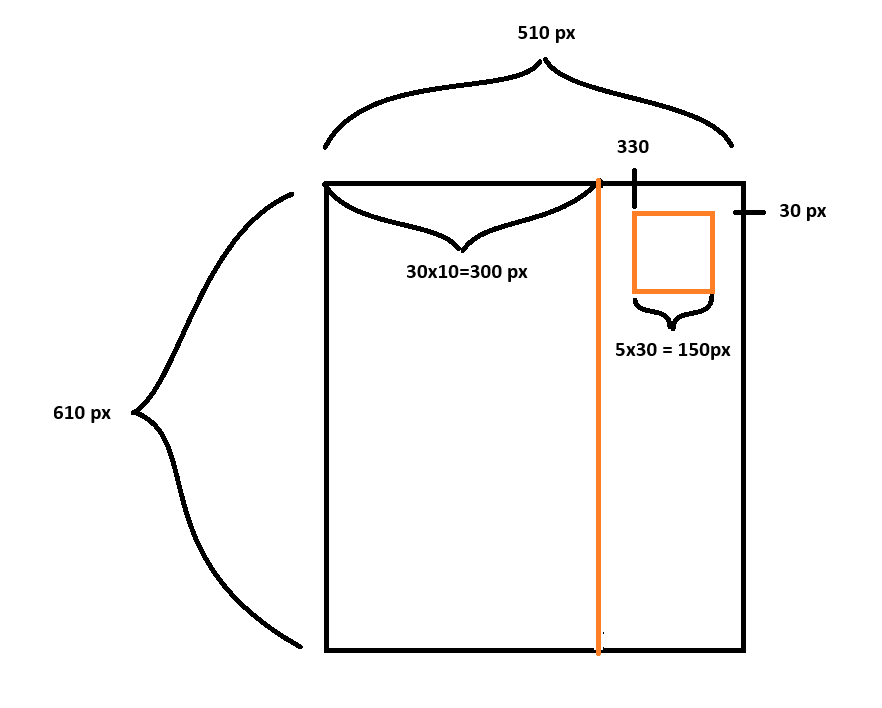
\includegraphics[scale=0.5]{dessin_coordonnees.png}
\caption{\label{dessin6} Schéma représentatif du plateau}
\end{figure}
Cette méthode de visualisation du plateau sera utilisée tout au long du programme dans les cas où il faudra compter en pixel des coordonnées.
\\\\
De la ligne \textcolor{gris}{17} à la ligne \textcolor{gris}{26} nous avons une double boucle for.
\begin{lstlisting}
for(i=0;i<20;i++)
    {
      for(j=0;j<10;j++)
	{
	  if(g->tet->matrix[i][j]=='1')
	    {
	      mino_display(g,g->tet->current_type,i,j);
	    }
	}
    }
\end{lstlisting}
Elle permet de parcourir la matrice et d'afficher un mino coloré la où la case de la matrice est remplie. Nous utilisons donc une condition pour détecter si la case pointer par g->tet->matrix[i][j] est remplie. Si c'est le cas alors nous dessinons un mino à cet emplacement avec le fonction
\begin{equation*}
    \text{mino\_display(g,g->tet->current\_type,i,j); \ref{mino.c}}
\end{equation*}
qui dessinera le mino en fonction du type du mino présent dans le buffer. Cela aura pour effet de transformer tous les minos de la matrice en une couleur unique. Nous n'avons pas trouvé d'autre solution.
\\\\
La suite du programme est une répétition de la fonction mino\_display de façons conditionnée afin d'afficher le tetrimino présent dans le buffer. Il y aura donc une condition pour chaque types en fonction du pointeur g->tet->current\_type et dans ces conditions, des conditions pour chaque rotation en fonction du pointeur g->tet->current\_rotation.
\\
Prenons pour exemple le tetrimino I à la rotation 0 :
\begin{lstlisting}
if(g->tet->current_type==0)
    {//Tetrimino I
      if(g->tet->current_rotation==0)
	{//Rotation 0
	  mino_display(g,g->tet->current_type,g->tet->current_line,g->tet->current_column-1);
	  mino_display(g,g->tet->current_type,g->tet->current_line,g->tet->current_column);
	  mino_display(g,g->tet->current_type,g->tet->current_line,g->tet->current_column+1);
	  mino_display(g,g->tet->current_type,g->tet->current_line,g->tet->current_column+2);
	}
\end{lstlisting}
Ligne \textcolor{gris}{1} nous avons la première condition. g->tet->current\_type peut être égale à 0, 1, 2, 3, 4, 5, ou 6 qui correspond aux valeurs du type associé au tetrimino que nous avons décrit dans le fichier tetris.c \ref{tetrimino}. Les types associés respectent l'énumération présente dans le fichier tetris.h \ref{tetris.h}.
\\
\\La ligne \textcolor{gris}{3} décrit la rotation du tetrimino ou g->tet->current\_rotation peut être égale à 0, 1, 2 ou 3, d'écrites également dans le fichier tetris.c.
\\
\\Enfin nous avons quatre utilisations de la fonction mino\_display \ref{mino_display}, un par mino et tous les tetriminos sont constitués de quatre minos. La fonction prendra donc en paramètre ligne et colonne l'emplacement du mino dans le buffer. Pour se faire il faudra passer par une conversion de g->tet->current\_line et g->tet->current\_column.
\\Pour cela il a fallu passer par un dessin (nous rappelons que la ligne et la colonne est centré sur le centre du tableau des tetrimino).
\begin{figure}[ht]
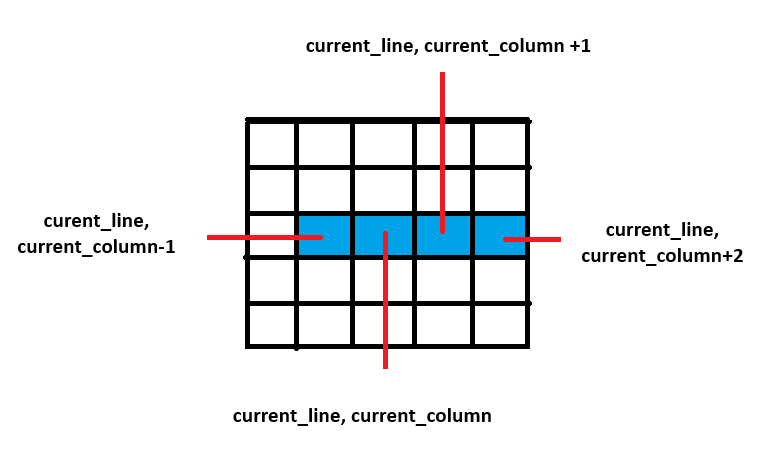
\includegraphics[scale=0.5]{tetrimino_dessin.png}
\caption{\label{dessin7} Schéma représentatif du tetrimino dans la matrice}
\end{figure}
\newpage
Nous réitérerons le processus pour tous les types et pour toutes les rotations et nous obtenons un affichage pour chaque tetrimino. 
\subsubsection{TODO n°2 : afficher le prochain tetrimino}
\label{todo2}
\begin{lstlisting}
if(g->tet->next_type==0)
    {//I
      //Déclaration d'un pointeur de type Color qui point vers les valeur rouge, vert et bleu d'une couleur.
      Color *color_I;
      
      //Allocation de mémoire pour la variable couleur.
      color_I = calloc(31,sizeof(Color));

      //Teste si l'allocation c'est bien passé.
      if(!color_I)
	return;

      //Affectation de la couleur à la variable. Pour l'obtenir on calcule le pourcentage de 255 et on soustrait par i*8.5 pour avoir 30 couleur différente. 30 pour le nombre de pixel.
      for(i=0;i<30;i++)// 255/30=8.5
	{
	  color_I[i].r=0;
	  color_I[i].g=255-(i*8.5);
	  color_I[i].b=255-(i*8.5);
	}

      //Affichage de chaque mino, en haut à droite, en fonction de leur position en pixel.
      for(i=0;i<30;i++)
	{
	  SDL_SetRenderDrawColor(g->ren,color_I[i].r,color_I[i].g,color_I[i].b,255);
	  for(j=i;j<30;j++)
	    {
	      SDL_RenderDrawPoint(g->ren,360+j,90+i);
	      SDL_RenderDrawPoint(g->ren,390+j,90+i);
	      SDL_RenderDrawPoint(g->ren,420+j,90+i);
	      SDL_RenderDrawPoint(g->ren,450+j,90+i);
	      
	    }
	  for(z=i+1;z<30;z++)
	    {
	      SDL_RenderDrawPoint(g->ren,360+i,90+z);
	      SDL_RenderDrawPoint(g->ren,390+i,90+z);
	      SDL_RenderDrawPoint(g->ren,420+i,90+z);
	      SDL_RenderDrawPoint(g->ren,450+i,90+z);
	    }

	}
    }
  else if(g->tet->next_type==1)
    {
      Color *color_J;
      color_J = calloc(31,sizeof(Color));
      if(!color_J)
	return;

      for(i=0;i<30;i++)
	{
	  color_J[i].r=0;
	  color_J[i].g=0;
	  color_J[i].b=255-i*8.5;
	}
      for(i=0;i<30;i++)
	{
	  SDL_SetRenderDrawColor(g->ren,color_J[i].r,color_J[i].g,color_J[i].b,255);
	  for(j=i;j<30;j++)
	    {
	      SDL_RenderDrawPoint(g->ren,360+j,60+i);
	      SDL_RenderDrawPoint(g->ren,360+j,90+i);
	      SDL_RenderDrawPoint(g->ren,390+j,90+i);
	      SDL_RenderDrawPoint(g->ren,420+j,90+i);
	      
	    }
	  for(z=i+1;z<30;z++)
	    {
	      SDL_RenderDrawPoint(g->ren,360+i,60+z);
	      SDL_RenderDrawPoint(g->ren,360+i,90+z);
	      SDL_RenderDrawPoint(g->ren,390+i,90+z);
	      SDL_RenderDrawPoint(g->ren,420+i,90+z);
	    }

	}
    }
  else if(g->tet->next_type==2)
    {
      Color *color_L;
      color_L = calloc(31,sizeof(Color));
      if(!color_L)
	return;

      for(i=0;i<30;i++)
	{
	  color_L[i].r=255-i*8.5;
	  color_L[i].g=165.75-i*5.525;
	  color_L[i].b=0;
	}
      for(i=0;i<30;i++)
	{
	  SDL_SetRenderDrawColor(g->ren,color_L[i].r,color_L[i].g,color_L[i].b,255);
	  for(j=i;j<30;j++)
	    {
	      SDL_RenderDrawPoint(g->ren,360+j,90+i);
	      SDL_RenderDrawPoint(g->ren,390+j,90+i);
	      SDL_RenderDrawPoint(g->ren,420+j,90+i);
	      SDL_RenderDrawPoint(g->ren,420+j,60+i);
	      
	    }
	  for(z=i+1;z<30;z++)
	    {
	      SDL_RenderDrawPoint(g->ren,360+i,90+z);
	      SDL_RenderDrawPoint(g->ren,390+i,90+z);
	      SDL_RenderDrawPoint(g->ren,420+i,90+z);
	      SDL_RenderDrawPoint(g->ren,420+i,60+z);
	    }

	}
    }
  else if(g->tet->next_type==3)
    {
      Color *color_O;
      color_O = calloc(31,sizeof(Color));
      if(!color_O)
	return;

      for(i=0;i<30;i++)
	{
	  color_O[i].r=255-i*8.5;
	  color_O[i].g=255-i*8.5;
	  color_O[i].b=0;
	}
      for(i=0;i<30;i++)
	{
	  SDL_SetRenderDrawColor(g->ren,color_O[i].r,color_O[i].g,color_O[i].b,255);
	  for(j=i;j<30;j++)
	    {
	      SDL_RenderDrawPoint(g->ren,390+j,90+i);
	      SDL_RenderDrawPoint(g->ren,420+j,90+i);
	      SDL_RenderDrawPoint(g->ren,390+j,120+i);
	      SDL_RenderDrawPoint(g->ren,420+j,120+i);
	      
	    }
	  for(z=i+1;z<30;z++)
	    {
	      SDL_RenderDrawPoint(g->ren,390+i,90+z);
	      SDL_RenderDrawPoint(g->ren,420+i,90+z);
	      SDL_RenderDrawPoint(g->ren,390+i,120+z);
	      SDL_RenderDrawPoint(g->ren,420+i,120+z);
	    }
	}
      
    }
  else if(g->tet->next_type==4)
    {
      Color *color_S;
      color_S = calloc(31,sizeof(Color));
      if(!color_S)
	return;

      for(i=0;i<30;i++)
	{
	  color_S[i].r=0;
	  color_S[i].g=127.5-i*4.25;
	  color_S[i].b=0;
	}
      for(i=0;i<30;i++)
	{
	  SDL_SetRenderDrawColor(g->ren,color_S[i].r,color_S[i].g,color_S[i].b,255);
	  for(j=i;j<30;j++)
	    {
	      SDL_RenderDrawPoint(g->ren,360+j,90+i);
	      SDL_RenderDrawPoint(g->ren,390+j,90+i);
	      SDL_RenderDrawPoint(g->ren,390+j,60+i);
	      SDL_RenderDrawPoint(g->ren,420+j,60+i);
	      
	    }
	  for(z=i+1;z<30;z++)
	    {
	      SDL_RenderDrawPoint(g->ren,360+i,90+z);
	      SDL_RenderDrawPoint(g->ren,390+i,90+z);
	      SDL_RenderDrawPoint(g->ren,390+i,60+z);
	      SDL_RenderDrawPoint(g->ren,420+i,60+z);
	    }
	}
    }
  else if(g->tet->next_type==5)
    {
      Color *color_T;
      color_T = calloc(31,sizeof(Color));
      if(!color_T)
	return;

      for(i=0;i<30;i++)
	{
	  color_T[i].r=237.15-i*7.905;
	  color_T[i].g=130.05-i*4.335;
	  color_T[i].b=237.15-i*7.905;
	}
      for(i=0;i<30;i++)
	{
	  SDL_SetRenderDrawColor(g->ren,color_T[i].r,color_T[i].g,color_T[i].b,255);
	  for(j=i;j<30;j++)
	    {
	      SDL_RenderDrawPoint(g->ren,360+j,90+i);
	      SDL_RenderDrawPoint(g->ren,390+j,90+i);
	      SDL_RenderDrawPoint(g->ren,390+j,60+i);
	      SDL_RenderDrawPoint(g->ren,420+j,90+i);
	      
	    }
	  for(z=i+1;z<30;z++)
	    {
	      SDL_RenderDrawPoint(g->ren,360+i,90+z);
	      SDL_RenderDrawPoint(g->ren,390+i,90+z);
	      SDL_RenderDrawPoint(g->ren,390+i,60+z);
	      SDL_RenderDrawPoint(g->ren,420+i,90+z);
	    }
	}
      
    }
  else if(g->tet->next_type==6)
    {
      Color *color_Z;
      color_Z = calloc(31,sizeof(Color));
      if(!color_Z)
	return;

      for(i=0;i<30;i++)
	{
	  color_Z[i].r=255-i*8.5;
	  color_Z[i].g=0;
	  color_Z[i].b=0;
	}
      for(i=0;i<30;i++)
	{
	  SDL_SetRenderDrawColor(g->ren,color_Z[i].r,color_Z[i].g,color_Z[i].b,255);
	  for(j=i;j<30;j++)
	    {
	      SDL_RenderDrawPoint(g->ren,360+j,60+i);
	      SDL_RenderDrawPoint(g->ren,390+j,60+i);
	      SDL_RenderDrawPoint(g->ren,390+j,90+i);
	      SDL_RenderDrawPoint(g->ren,420+j,90+i);
	      
	    }
	  for(z=i+1;z<30;z++)
	    {
	      SDL_RenderDrawPoint(g->ren,360+i,60+z);
	      SDL_RenderDrawPoint(g->ren,390+i,60+z);
	      SDL_RenderDrawPoint(g->ren,390+i,90+z);
	      SDL_RenderDrawPoint(g->ren,420+i,90+z);
	    }
	}
    }
\end{lstlisting}
\newpage
Dans cette partie du code nous avons également une répétition de condition pour chaque types de tetrimino, nous allons en prendre l'exemple du tetrimino J et le commenter.
\begin{lstlisting}
else if(g->tet->next_type==1)
    {
      Color *color_J;
      color_J = calloc(31,sizeof(Color));
      if(!color_J)
	return;

      for(i=0;i<30;i++)
	{
	  color_J[i].r=0;
	  color_J[i].g=0;
	  color_J[i].b=255-i*8.5;
	}
      for(i=0;i<30;i++)
	{
	  SDL_SetRenderDrawColor(g->ren,color_J[i].r,color_J[i].g,color_J[i].b,255);
	  for(j=i;j<30;j++)
	    {
	      SDL_RenderDrawPoint(g->ren,360+j,60+i);
	      SDL_RenderDrawPoint(g->ren,360+j,90+i);
	      SDL_RenderDrawPoint(g->ren,390+j,90+i);
	      SDL_RenderDrawPoint(g->ren,420+j,90+i);
	      
	    }
	  for(z=i+1;z<30;z++)
	    {
	      SDL_RenderDrawPoint(g->ren,360+i,60+z);
	      SDL_RenderDrawPoint(g->ren,360+i,90+z);
	      SDL_RenderDrawPoint(g->ren,390+i,90+z);
	      SDL_RenderDrawPoint(g->ren,420+i,90+z);
	    }

	}
\end{lstlisting}
Nous pouvons remarquer que le code a des similitudes avec le code de mino\_display() \ref{mino_display}.
\\Ligne \textcolor{gris}{1}, la condition en fonction du type.
\\\\
De la ligne \textcolor{gris}{3} à la ligne \textcolor{gris}{6}, nous initialisons un pointeur de type Color pour le tetrimino J \ref{mino.h}, ensuite nous allouons une quantité de mémoire égale à 31 x sizeof(Color) pour stocker dans Color\_J 30 valeurs d'une couleur allant du plus claire au plus sombre, une par ligne de pixel. Nous effectuons également un teste pour vérifier que l'allocation a correctement fonctionné.
\\\\
De la ligne \textcolor{gris}{8} à la ligne \textcolor{gris}{13}, nous stockons dans color\_J nos 30 couleurs. Le tableau aura une couleur allant du plus claire au plus sombre.
\\Il a fallu effectuer quelques calcules pour avoir le bon résultat. Le premiers est de diviser 255 par 30 ce qui donne 8.5, ainsi nous aurons 30 valeurs pour 30 intensités.
\\Le deuxième nécessite un calcule de pourcentage. A l'aide du liens \href{https://en.wikipedia.org/wiki/X11_color_names#Derived_lists}{wikipédia} présent sur le pdf du projet, nous avons calculé pour chaque couleurs du tétrimino la valeur en pourcentage de l'indice de couleur 255. Dans le cas du tetrimino J la couleur étant le bleu nous avons comme rouge = 0\%, vert = 0\% et bleu = 100\% et 100\% de 255 est égale à 255, mais pour des cas plus compliqués, il faut utiliser la formule suivante :
\begin{equation}
    \frac{\text{veleur} \times \text{pourcentage}}{100}
\end{equation}
Nous avons donc utilisé cette formule pour chaque couleurs.
\\\\
Ensuite nous avons une boucle for principale dans laquelle il y a deux boucles for différentes.
\\La boucle for principale permet de parcourir les 30 intensité de color\_J et d'avoir 30 itération, une par ligne de pixel.
\\le seconde boucle for permet de dessiner pixel par pixel les lignes en commencent sur la diagonal du mino, allant de l'intensité la plus claire à la plus sombre. Pour cela nous avons utilisé la commande :
\begin{equation*}
    \text{SDL\_RenderDarwPoint(renderer,x,y);}
\end{equation*}
qui dessine une pixel aux coordonnées x et y et il a fallu affecter à j la valeur i pour bien commencer à la valeur sur la diagonal de notre mino. Par la suite l'incrémentation de j par la boucle for, nous permettra de bien parcourir tous les pixels de la ligne i.
\\Une chose à préciser, lors de la conception du code, nous voulions à l'origine dessiner ligne par ligne le mino, mais le code semblait plus compliqué, voir potentiellement infaisable. Nous avons donc préféré garder la méthode des pixels afin de ne pas perdre trop de temps si le codage n'était pas possible.
\newpage 
Dans notre cas il fallait identifier les coordonnées x et y pour. Pour cela nous sommes passés par un dessin.
\begin{figure}[ht]
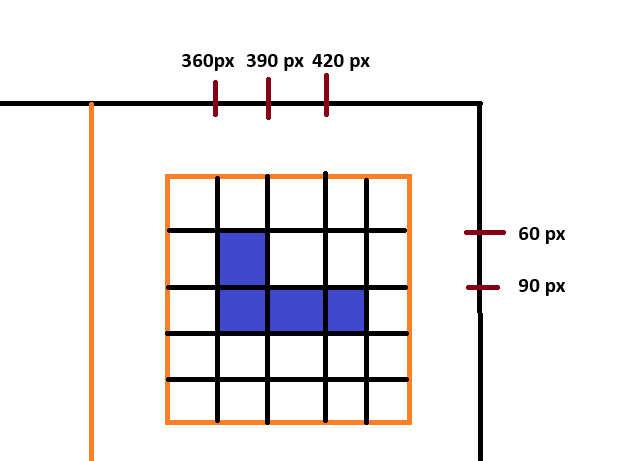
\includegraphics[scale=0.5]{dessin3.png}
\caption{\label{dessin8} Schéma du tetrimino suivant}
\end{figure}
La figure ci-dessus est une zoome sur le premiers schéma \ref{dessin1}
\\\\Nous avons donc utilisé cette méthode d'identification pour chaque tetrimino.
\\Enfin la dernière boucle permet de dessiner les colonnes du mino en commencent à la ligne en dessous de la diagonal. Donc cette fois ci ce sera les coordonnées des colonnes qu'il faudra incrémenter de 1, et pour bien respecter le premier pixel situé en-dessous de la diagonal, nous affectons la valeur i+1 à z.
\\
Finalement pour obtenir le dessins d'un tetrimino il faut répéter 4 fois le dessin des pixels pour chaque coins supérieurs gauches du mino, en tenant compte des positions des minos, en fonction du type de tetrimino.
\subsubsection{TODO n°3 : afficher le score, le niveau et le nombre de lignes eliminées}
\label{todo3}
Dans cette section nous nous sommes beaucoup aider du tutoriel de Cam sur youtube dans la \href{https://www.youtube.com/watch?v=NQZNHUoba-8}{partie 1} et la \href{https://www.youtube.com/watch?v=LS_eeI-9-pA}{partie 2} sur l'utilisation de TTF\_font pour programmer l'affichage du score, du niveau et du nombre de ligne.
\begin{lstlisting}
 //Déclaration nécessaire:
  //Variable de la donnée
  int score = g->tet->score;
  //Tableau contenant la donnée
  char buffer_s[20]={'\0'};
  
  int level = g->tet->level;
  char buffer_l[2]={'\0'};
  
  int nbr_lines = g->tet->nbr_lines;
  char buffer_nl[10]={'\0'};

  //Tableau contenant la donnée et un texte
  char final_buffer_s[26]={'\0'};
  char final_buffer_l[8]={'\0'};
  char final_buffer_nl[20]={'\0'};

  // Ici on déclare des surfaces qui permetrons d'écrire le texte,
  // à l'aide de la fonction TTF_RenderText_Solid().
  SDL_Surface * text_s= NULL;
  SDL_Surface * text_l= NULL;
  SDL_Surface * text_nl= NULL;

  //Ici nous déclarons des texture dans lesquelles seront copiées les surfaces.
  SDL_Texture * texture_s = NULL;
  SDL_Texture * texture_l = NULL;
  SDL_Texture * texture_nl = NULL;

  //Il s'agit ici de réctangle représentant la surface dans laquelle il y aura le texte.
  SDL_Rect rect_s = {300,210,210,30};
  SDL_Rect rect_l = {300,240,210,30};
  SDL_Rect rect_nl = {300,270,210,30};

  // On une couleur
  SDL_Color white = {255,255,255,255};  
  

  // Ici itoa transforme une valeur numérique en une chaine de carractère et on la mets dans le tableau.
  itoa(score,buffer_s,10);
  itoa(level,buffer_l,10);
  itoa(nbr_lines,buffer_nl,10);

  //Avec strcpy on copie "score:" dans le buffer final.
  strcpy(final_buffer_s,"Score:");
  //Avec strcat on concatène les tableau de carractère.
  strcat(final_buffer_s,buffer_s);
  
  strcpy(final_buffer_l,"level:");
  strcat(final_buffer_l,buffer_l);
  
  strcpy(final_buffer_nl,"nbr_lines:");
  strcat(final_buffer_nl,buffer_nl);

  
  //Ici on "met" dans la surface les chaine de caractère et on teste l'erreur.
  text_s = TTF_RenderText_Solid(g->font, final_buffer_s,white);
  if(!text_s)
    {
      //En cas d'erreur on libert toutes les allocation de mémoire.
      SDL_FreeSurface(text_s);
      TTF_CloseFont(g->font);
      SDL_LogError(SDL_LOG_CATEGORY_APPLICATION, "error : %s\n", SDL_GetError());
      SDL_DestroyRenderer(g->ren);
      SDL_DestroyWindow(g->win);
      TTF_Quit();
      SDL_Quit();
      return;
    }

  text_l = TTF_RenderText_Solid(g->font, final_buffer_l,white);
  if(!text_l)
    {
      SDL_FreeSurface(text_l);
      TTF_CloseFont(g->font);
      SDL_LogError(SDL_LOG_CATEGORY_APPLICATION, "error : %s\n", SDL_GetError());
      SDL_DestroyRenderer(g->ren);
      SDL_DestroyWindow(g->win);
      TTF_Quit();
      SDL_Quit();
      return;
    }

  text_nl = TTF_RenderText_Solid(g->font, final_buffer_nl,white);
  if(!text_nl)
    {
      SDL_LogError(SDL_LOG_CATEGORY_APPLICATION, "error : %s\n", SDL_GetError());
      SDL_FreeSurface(text_nl);
      TTF_CloseFont(g->font);
      SDL_DestroyRenderer(g->ren);
      SDL_DestroyWindow(g->win);
      TTF_Quit();
      SDL_Quit();
      return;
    }

  //Ensuite on créer des texture à partir des surface, car la texture nous permetra d'avoir l'affichage souhaité.
  texture_s = SDL_CreateTextureFromSurface(g->ren,text_s);
  SDL_FreeSurface(text_s);
  //On teste l'erreur.
  if((!texture_s) || (SDL_QueryTexture(texture_s,NULL,NULL,&rect_s.w,&rect_s.h) !=0) )
    {
      SDL_LogError(SDL_LOG_CATEGORY_APPLICATION, "error : %s\n", SDL_GetError());
      TTF_CloseFont(g->font);
      SDL_DestroyTexture(texture_s);
      SDL_DestroyRenderer(g->ren);
      SDL_DestroyWindow(g->win);
      TTF_Quit();
      SDL_Quit();
      return;
    }
     
  texture_l = SDL_CreateTextureFromSurface(g->ren,text_l);
  SDL_FreeSurface(text_l);
  if((!texture_l) || (SDL_QueryTexture(texture_l,NULL,NULL,&rect_l.w,&rect_l.h) !=0))
    {
      SDL_LogError(SDL_LOG_CATEGORY_APPLICATION, "error : %s\n", SDL_GetError());
      TTF_CloseFont(g->font);
      SDL_DestroyTexture(texture_l);
      SDL_DestroyRenderer(g->ren);
      SDL_DestroyWindow(g->win);
      TTF_Quit();
      SDL_Quit();
      return;
    }
  
  texture_nl = SDL_CreateTextureFromSurface(g->ren,text_nl);
  SDL_FreeSurface(text_nl);
  if((!texture_nl) || (SDL_QueryTexture(texture_nl,NULL,NULL,&rect_nl.w,&rect_nl.h) !=0))
    {
      SDL_LogError(SDL_LOG_CATEGORY_APPLICATION, "error : %s\n", SDL_GetError());
      TTF_CloseFont(g->font);
      SDL_DestroyTexture(texture_nl);
      SDL_DestroyRenderer(g->ren);
      SDL_DestroyWindow(g->win);
      TTF_Quit();
      SDL_Quit();
      return;
    }

  //On va afficher le texte en associant la texture au renderer pour avoir un affichage.
  if (SDL_RenderCopy(g->ren, texture_s,NULL,&rect_s) != 0)
    {
      SDL_LogError(SDL_LOG_CATEGORY_APPLICATION, "error : %s\n", SDL_GetError());
      TTF_CloseFont(g->font);
      SDL_DestroyTexture(texture_s);
      SDL_DestroyTexture(texture_l);
      SDL_DestroyTexture(texture_nl);
      SDL_DestroyRenderer(g->ren);
      SDL_DestroyWindow(g->win);
      TTF_Quit();
      SDL_Quit();
      return;
    }
  
  if (SDL_RenderCopy(g->ren, texture_l,NULL,&rect_l) != 0)
    {
      SDL_LogError(SDL_LOG_CATEGORY_APPLICATION, "error : %s\n", SDL_GetError());
      TTF_CloseFont(g->font);
      SDL_DestroyTexture(texture_s);
      SDL_DestroyTexture(texture_l);
      SDL_DestroyTexture(texture_nl);
      SDL_DestroyRenderer(g->ren);
      SDL_DestroyWindow(g->win);
      TTF_Quit();
      SDL_Quit();
      return;
    }

  if (SDL_RenderCopy(g->ren, texture_nl,NULL,&rect_nl) != 0)
    {
      SDL_LogError(SDL_LOG_CATEGORY_APPLICATION, "error : %s\n", SDL_GetError());
      TTF_CloseFont(g->font);
      SDL_DestroyTexture(texture_s);
      SDL_DestroyTexture(texture_l);
      SDL_DestroyTexture(texture_nl);
      SDL_DestroyRenderer(g->ren);
      SDL_DestroyWindow(g->win);
      TTF_Quit();
      SDL_Quit();
      return;
    }

  //On affecte aux pointeur de texture les texture d'affichage.
  g->tex_s=texture_s;
  g->tex_l=texture_l;
  g->tex_nl=texture_nl;

  //On détruit les texture d'affichage inutile.
  SDL_DestroyTexture(texture_s);
  SDL_DestroyTexture(texture_l);
  SDL_DestroyTexture(texture_nl);

  //Affichage du résultat.
  SDL_RenderPresent(g->ren);

  update = 0;
  
}
\end{lstlisting}
Dans ce programme, nous effectuons 3 fois le même méthode d'affichage. Pour la décrire, nous allons donc d'abord présenter les déclarations qui sont différentes, puis décrire la création de l'affichage du score qui sera différente des autre par ces coordonnées de placement et son contenue.
\begin{lstlisting}
  //Variable de la donnée
  int score = g->tet->score;
  //Tableau contenant la donnée
  char buffer_s[20]={'\0'};
  
  int level = g->tet->level;
  char buffer_l[2]={'\0'};
  
  int nbr_lines = g->tet->nbr_lines;
  char buffer_nl[10]={'\0'};

  //Tableau contenant la donnée et un texte
  char final_buffer_s[26]={'\0'};
  char final_buffer_l[8]={'\0'};
  char final_buffer_nl[20]={'\0'};
\end{lstlisting}
Dans ce début de partie du programme nous initialisons des variabales contenant les valeurs de score, nbr\_line et level afin de faciliter le codage. Ensuite nous créons des tableaux nommés "buffer" pour contenir les valeurs respectivement associées. Ensuite nous créons également des tableaux nommés "final\_buffer" qui contiendront à la fois les datas associées et le texte d'affichage. Le nombre de valeur de ces tableaux est défini par le nombre de char qu'il contiennent. Pour le buffer de score et de nbr\_line l'affichage est limité.
\\\\
Passons à l'affichage de score.
\begin{lstlisting}
int score = g->tet->score;
char buffer_s[20]={'\0'};
char final_buffer_s[26]={'\0'};
SDL_Surface * text_s= NULL;
SDL_Texture * texture_s = NULL;
SDL_Rect rect_s = {300,210,210,30};
SDL_Color white = {255,255,255,255};  

itoa(score,buffer_s,10);
strcpy(final_buffer_s,"Score:");
strcat(final_buffer_s,buffer_s);

text_s = TTF_RenderText_Solid(g->font, final_buffer_s,white);
  if(!text_s)
    {
      SDL_FreeSurface(text_s);
      TTF_CloseFont(g->font);
      SDL_LogError(SDL_LOG_CATEGORY_APPLICATION, "error : %s\n", SDL_GetError());
      SDL_DestroyRenderer(g->ren);
      SDL_DestroyWindow(g->win);
      TTF_Quit();
      SDL_Quit();
      return;
    }

texture_s = SDL_CreateTextureFromSurface(g->ren,text_s);
  SDL_FreeSurface(text_s);
  if((!texture_s) || (SDL_QueryTexture(texture_s,NULL,NULL,&rect_s.w,&rect_s.h) !=0) )
    {
      SDL_LogError(SDL_LOG_CATEGORY_APPLICATION, "error : %s\n", SDL_GetError());
      TTF_CloseFont(g->font);
      SDL_DestroyTexture(texture_s);
      SDL_DestroyRenderer(g->ren);
      SDL_DestroyWindow(g->win);
      TTF_Quit();
      SDL_Quit();
      return;
    }

if (SDL_RenderCopy(g->ren, texture_s,NULL,&rect_s) != 0)
    {
      SDL_LogError(SDL_LOG_CATEGORY_APPLICATION, "error : %s\n", SDL_GetError());
      TTF_CloseFont(g->font);
      SDL_DestroyTexture(texture_s);
      SDL_DestroyTexture(texture_l);
      SDL_DestroyTexture(texture_nl);
      SDL_DestroyRenderer(g->ren);
      SDL_DestroyWindow(g->win);
      TTF_Quit();
      SDL_Quit();
      return;
    }

g->tex_s=texture_s;

SDL_DestroyTexture(texture_s);
  
}
\end{lstlisting}
Premièrement nous devons initialiser une surface et une texture à NULL afin de pouvoir les utiliser plus tard.
\\Ensuite nous avons besoin d'initialiser un rectangle pour placer l'affichage à l'endroit voulu, qui est situé deux cases en dessous du rectangle orange du schéma 3 \ref{dessin3}. Donc en coordonnée 300 et 210 de taille 210x30 pour recouvrir la ligne.
\\Enfin nous initialisons également la couleur du texte qui sera blanc.
\\\\
Ensuite des lignes \textcolor{gris}{9} à \textcolor{gris}{11} nous créons un tableau affichant "Score :[le score]".
\\Pour cela nous utilisons la fonction \href{https://www.ibm.com/docs/fr/i/7.5?topic=functions-itoa-convert-integer-string}{itoa} qui permet de convertir des chiffres en lignes de caractères et de stocker le résultat dans un espace de mémoire de type char. Dans notre cas la valeur numérique est "score", la mémoire est "buffer\_s" et 10 représente la base numérique, qui est décimal dans notre cas.
\\Par la suite nous utilisons \href{https://www.ibm.com/docs/fr/i/7.5?topic=functions-strcpy-copy-strings}{strcpy} qui copie une chaîne de caractère dans un espace de mémoire de type char et donc nous copions "Score :" dans le buffer final.
\\Et nous ajoutons buffer\_s dans final\_buffer\_s avec \href{https://www.ibm.com/docs/fr/i/7.5?topic=functions-strcat-concatenate-strings}{strcat}.
\\\\
De la ligne \textcolor{gris}{13} à \textcolor{gris}{24}, nous "écrivons" dans la surface le texte en allouant de la mémoire pour cela on utilise la fonction 
\begin{equation*}
\text{TTF\_RenderText\_Solid(TTF\_font\  *font,char\  *text, SDL\_Color color);}
\end{equation*}
On pourra avec ça écrire dans la surface text\_s le texte présent dans final\_buffer\_s, en blanc avec la police pointée par g->font qui est "arial".
\\Nous testons également si l'allocation de mémoire à bien été effectuée, si l'allocation échoue il faut libérer toutes les allocations de mémoire précédemment allouées, renvoyer une erreur, quitter le SDL et TTF à l'aide des commande respective.
\\\\Ensuite ligne \textcolor{gris}{26} nous créons une texture\_s depuis une surface. Cela nous permettra de manipuler plus facilement le texte à afficher. Nous utilisons alors la commande :
\begin{equation*}
\text{SDL\_CreateTextureFromSurface(g->ren,text\_s);}
\end{equation*}
On libère parla suite la mémoire allouée par la surface. Également, si l'allocation de mémoire échoue, il faut agir en conséquence.
\\Nous allons également charger le texte en mémoire avec la deuxième partie de la condition, ce qui est nécessaire pour son affichage. On utilise pour cela
\begin{equation*}
    \text{SDL\_QueryTexture(texture\_s,NULL,NULL,\&rect\_s.w,\& rect\_s.h)}
\end{equation*}
Puis nous affichons le texte avec un if et la commande 
\begin{equation*}
\text{SDL\_RenderCopy(g->ren,texture\_s,NULL,\&rect\_s);}
\end{equation*}
Ici aussi si le teste est faut il faut bien libérer la mémoire et quitter à la fois la SDL et TTF.
\\\\
Enfin on affecte au pointeur g->tex\_s la texture\_s pour pouvoirs libérer la mémoire de la texture\_s et une fois le jeu fermé, libérer la mémoire de g->tex\_s grâce à la fonction game\_del() \ref{game_del}.
\subsection{game\_new()}
\label{game_new}
La fonction game\_new() prend en argument deux int un pour la coordonnée x et l'autre pour la coordonnée y du coin supérieure gauche de la fenêtre. Elle renvoie de façons générale un nouveau jeu en ouvrant une fenêtre, en créent un rendu, un font, un pointeur sur un nouveau Tetris et en obtenant des valeurs nécessaires au bon fonctionnement du jeux.
\\Initialement nous ne savions pas comment faire pointer g->win, g->ren, g->font, g->freq et g->count. Nous avions laissé ce travail pour plus tard pour avancer et surtout parce que nous pension que c'etait inutile de le faire. Plus tard après l'étude de la SDL, nous avons compris comment le faire et pourquoi le faire, car c'est en réalité dans cette fonction même que le jeux est créé et donc il s'agit de l'unique emplacement de leur création.
\begin{lstlisting}
Game *game_new(int x, int y)
{
  int w=510;
  int h=600;
  Game *g;
  g=malloc(sizeof(Game));

  if(!g)
    return NULL;

  //On affecte les textures à NULL, car elle ne sont utile que dans la fonction game_board_update.
  g->tex_s=NULL;
  g->tex_l=NULL;
  g->tex_nl=NULL;

  g->tet_offset_x=x;

  g->tet_offset_y=y;

  //Affectation d'un nouvelle fenêtre.
  g->win = SDL_CreateWindow("Tetris",g->tet_offset_x,g->tet_offset_y , w, h, SDL_WINDOW_SHOWN);
  //On teste l'erreur.
  if (!g->win)
    {
      SDL_LogError(SDL_LOG_CATEGORY_APPLICATION, "error : %s\n", SDL_GetError());
      SDL_Quit();
      TTF_Quit();
      return NULL;
    }
  
  //Affectation d'un renderer.
  g->ren = SDL_CreateRenderer(g->win, -1, SDL_RENDERER_ACCELERATED);
  if(!g->ren)
    {
      SDL_LogError(SDL_LOG_CATEGORY_APPLICATION, "error : %s\n", SDL_GetError());
      SDL_DestroyWindow(g->win);
      SDL_Quit();
      TTF_Quit();
      return NULL;
    }

  //Affectation de la bibliothèque "arial" à g->font
  g->font =  TTF_OpenFont("font/arial.ttf",25);
  if(!g->font)
    {
      SDL_LogError(SDL_LOG_CATEGORY_APPLICATION, "error : %s\n", SDL_GetError());
      TTF_CloseFont(g->font);
      TTF_Quit();
      SDL_Quit();
      return NULL;
    }
      

  g->tet = tetris_new();


  g->mino_size=30;

  //Permet d'avoir la valeur du conteur de haute résolution en seconde
  g->freq = SDL_GetPerformanceFrequency();
  //Permet d'avoir la valeur du conteur de haute résolution
  g->count = SDL_GetPerformanceCounter();
  
  return g;
}
\end{lstlisting}
Premièrement on définit la hauteur et la largeur de la fenêtre avec l'initialisation de w et h. Ensuite on déclare un pointeur g vers la structure Game \ref{game.h} pour la quelle on alloue de la mémoire. Et nous testons si la mémoire à bien été allouée.
\\\\
Ligne \textcolor{gris}{12}, \textcolor{gris}{13} et \textcolor{gris}{14} on pointe les textures vers NULL car on leur affectera une mémoire dans la fonction game\_board\_update().
\\\\g->tet\_offset\_x et g->tet\_offset\_y point respectivement vers x et y pour le coin supérieur gauche de la fenêtre.
\\\\g->win pointe vers une fenêtre créer par la commande
\begin{equation*}
\text{SDL\_CreateWindow("Tetris",g->tet\_offset\_x,g->tet\_offset\_y,w,h,SDL\_WINDOW\_SHOWN);}
\end{equation*}
SDL\_WINDOW\_SHOWN peut prendre d'autre valeurs mais nous gardons celle-la pour notre projet. On teste aussi l'allocation
\\\\
On fait également pointer g->ren vers SDL\_CreateRenderer(g->win,-1,SDL\_RENDERER\_ACCELERATED); et on teste l'allocation.
\\\\Pour g->font on utilise TTF\_OpenFont("font/arial.ttf",25); qui permet d'aller chercher dans les fichiers local la police arial en taille 25. On teste également l'erreur et agissons en conséquence.
\\\\On fait pointer g->tet vers un teris\_new(); \ref{tetris_new} et g->mino\_size vers 30 qui sera la taille en pixel d'un mino.
\\\\Pour finir g->freq point vers SDL\_GetPerformanceFrequency(); et g->count vers SDL\_GetPerformanceCounter();
\\Il est important de retrouner g à la fin.

\subsection{game\_del()}
\label{game_del}
Cette fonction prend en argument un pointeur sur la structure Game et permet de libérer toutes les mémoires allouées par ce pointeur et de quitter le SDL et TTF. Elle est utilisée uniquement dans la fonction main.c \ref{main.c}, car elle permet de fermer le jeu une fois la boucle de game\_run() "fini". Initialement lors du codage du jeu nous voulions libérer les mémoires et quitter SDL et TTF dans toutes les fonctions les utilisant, cependant après l'étude de la SDL, nous avons compris qu'elles n'étaient nécessaires qu'une fois (sans compter les testes d'échec d'allocation de mémoires), car les différentes commandes de la SDL et TTF doivent tourner en boucle pour que le jeu puisse continuer de fonctionner et donc il ne faut pas les détruire, ou quitter SDL ou TTF.
\\Le code de la fonction le suivant :
\begin{lstlisting}
void game_del(Game *g)
{
  //on libert toute la mémoire allouer par nos fonctions et on quite la TTF puis SDL.
  //l'ordre semble être important
  
  tetris_del(g->tet);
  
  SDL_DestroyTexture(g->tex_s);
  SDL_DestroyTexture(g->tex_l);
  SDL_DestroyTexture(g->tex_nl);

  TTF_CloseFont(g->font);
  
  SDL_DestroyRenderer(g->ren);
  
  SDL_DestroyWindow(g->win);
  
  free(g);

  TTF_Quit();

  SDL_Quit();
}
\end{lstlisting}
Comme mentionné dans le programme l'ordre de l'utilisation des commandes semble être important, car en TD nous avons vu que pour une structure contenant un pointeur, il était nécessaire d'abord de libérer la mémoire des données de la structure puis de libérer la mémoire du pointeur de structure, car il pouvait y avoir une perte de mémoire. Dans cette même logique nous avons préférer libérer les mémoires dans l'ordre de dépendance.
\\Donc nous commençons par libérer le pointeur sur tetris avec la fonction tetris\_del() \ref{tetris_del}, puis nous libérons les textures permettant d'afficher le score, le nombre de lignes détruites et le niveau avec la commande
\begin{equation*}
\text{SDL\_DestroyTexture(Texture);}
\end{equation*}
qui prend une texture en argument et libère la mémoire allouée par celle-ci. Nous commençons par cette mémoire la, car elle est utilisée dans le rendu et donc pour éviter toute possibilité de perte de mémoire, nous l'avons placer en premiers.
\\Ensuite nous libérons la mémoire allouée par le pointeur de font avec la commande
\begin{equation*}
\text{TTF\_CloseFont(g->font);}
\end{equation*}
\\Nous faisons la même chose pour le rendu et la fenêtre
\begin{equation*}
\begin{split}
\text{SDL\_DestroyRenderer(g->ren);}
\\
\\
\text{SDL\_DestroyWindow(g->win);}
\end{split}
\end{equation*}
Nous le faisons dans cet ordre pour éviter une possible perte de mémoire.\\
A l'issue de ces libérations on peut libérer en dernier la mémoire allouée par g. Et enfin une fois que toutes les mémoires sont libérées nous devons quitter TTF puis SDL.

\subsection{game\_run()}
\label{game_run}
La fonction prend en argument un pointeur de type Game et renvoie des évènements déclenchables manuellement par le joueur et des évènements continues propre au jeu. 
\\Cette fonction fait partie des dernières à avoir été codée car il nous fallait coder les fonctions de teste de tetrimino avant. Dès que nous avions codé ces fonctions nous sommes aussitôt passé a son codage. Cependant il a fallu trouver les notations pour les évènements associés aux flèches directionnelles, à la barre d'espace et à la touche échappe. Nous avions trouvé quelques réponses dans un forum qui utilisait la bibliothèque SDL puis nous avions deviné pour le reste. 
\\ Le plus compliqué dans cette fonction a été la fin, car il fallait comprendre où il fallait coder la ligne pour faire descendre le tetrimino en fonction du temps et comment enclencher la suite d'évènements associées à la destruction de ligne. De plus pour cette fonction il à fallu créer une fonction qui n'était pas mentionnée, il s'agit de la fonction
\begin{equation*}
\text{tetris\_matrix\_update(g->tet);}
\end{equation*}
\begin{lstlisting}
void game_run(Game *g)
{
  SDL_Event events;
  int running;
  int i;
  int j;

  running =1;

  while (running)
    {
      Uint64 c;

      while(SDL_PollEvent(&events))
	{
	  switch(events.type)
	    {
	    case SDL_QUIT:
	      {
		running =0;
		break;
	      }
	    case SDL_KEYDOWN:
	      {
		switch (events.key.keysym.sym)
		  {
		  case SDLK_q:
		    {
		      running = 0;
		      break;
		    }
		  case SDLK_ESCAPE:
		    {
		      running = 0;
		      break;
		    }
		  case SDLK_SPACE:
		    {
		      /*descendre immédiatement le tetrimino tout en bas et mettre à jour, si c'est possible. */
		      for(i=0;i<20;i++)
			{
			  if(tetris_can_go_down(g->tet)==1)
			    {
			      g->tet->current_line+=1;
			    }
			}
		      game_board_update(g);
		      break;
		    }
		  case SDLK_LEFT:
		    {
		      /* déplacer le tétrimino à gauche et mettre à jour, si c'est possible.*/
		      if(tetris_can_go_left(g->tet)==1)
			{
			  g->tet->current_column -= 1;
			  game_board_update(g);
			  break;
			}
		      else
			{
			  break;
			}
		    }
		  case SDLK_RIGHT:
		    {
		      /*déplacer le tétrimino à droite et mettre à jour, si c'est possible. */
		      if(tetris_can_go_right(g->tet)==1)
			{
			  g->tet->current_column += 1;
			  game_board_update(g);
			  break;
			}
		      else
			{
			  break;
			}
		    }
		  case SDLK_DOWN:
		    {
		      /* déscendre de une case le tétrimino et mettre à jour, si c'est possible. */
		      if(tetris_can_go_down(g->tet)==1)
			{
			  g->tet->current_line += 1;
			  game_board_update(g);
			  break;
			}
		      else
			{
			  break;
			}
		    }
		  case SDLK_UP:
		    {
		      /* faire pivoter le tétrimino dans le sens horaire et mettre à jour, si c'est possible. */
		      if(tetris_can_rotate_h(g->tet)==1)
			{
			  if(g->tet->current_rotation +1 == 4)
			    {
			      g->tet->current_rotation =0;
			    }
			  else
			    {
			      g->tet->current_rotation += 1;
			    }
			  game_board_update(g);
			  break;
			}
		      else
			{
			  break;
			}
		    }
		  case SDLK_n:
		    {
		      /* faire pivoter dans le sens anti_horaire et mettre à jour, si c'est possible. */
		      if(tetris_can_rotate_ah(g->tet)==1)
			{
			  if(g->tet->current_rotation -1 == -1)
			    {
			      g->tet->current_rotation =3;
			    }
			  else
			    {
			      g->tet->current_rotation -= 1;
			    }
			  game_board_update(g);
			  break;
			}
		      else
			{
			  break;
			}
		    }
		  }
		break;
	      }
	    }
	}
      c= SDL_GetPerformanceCounter();

      if (update)
	game_board_update(g);

      if ((float)(c - g->count)/g->freq > tetris_get_drop_speed(g->tet))
	{
	  g->count = c;
	  if (tetris_can_go_down(g->tet))
	    {
	      //Permet de faire desendre le tétriminos chaque seconde.
	      g->tet->current_line+=1;
	      game_board_update(g);
	    }

	  //Permet de mettre fin à la boucle infini et donc du jeux.
	  else if((!tetris_can_go_down(g->tet) && g->tet->current_line == 0) ||(!tetris_can_go_down(g->tet) && g->tet->current_line == 1))
	  {
	    running=0;
	  }

	  else
	    {
	      /*
	       * detecter si une ou plusieurs lignes doivent etre retirees
	       * si c est le cas, mettre a jour le score, le niveau
	       * et le nombre de lignes
	       */
	      //Variable de contage
	      int count;
	      int count_lines=0;
	      int count_lvl=1;

	      //(Peut aider pour sauvegarder les couleur des tetriminos)
	      //Permet de sauvegarder les tetrimino dans matrix.
	      tetris_matrix_update(g->tet);

	      //Compte si un ligne est remplie de mino.
	      for(i=-2;i<=2;i++)
		{
		  count=0;
		  for(j=0;j<10;j++)
		    {
		      if(g->tet->matrix[g->tet->current_line-i][j] =='1')
			{
			  count+=1;
			  if(count==10)
			    count_lines+=1;
			}
		    }
		}
	      
	      if(count_lines==0)
		{
		  //Label vers la fin de la fonction
		  goto exit;
		}
	      //Si des lignes sont remplies
	      else if(count_lines!=0)
		{
		  //Mise à jour du score
		  if(count_lines == 1)
		    {
		      g->tet->score += 100*g->tet->level;
		    }
		  else if(count_lines == 2)
		    {
		      g->tet->score += 300*g->tet->level;
		    }
		  else if(count_lines == 3)
		    {
		      g->tet->score += 500*g->tet->level;
		    }
		  else if(count_lines == 4)
		    {
		      g->tet->score += 800*g->tet->level;
		    }
		  
		  //Mise à jour de nbr_lines
		  g->tet->nbr_lines += count_lines;
		  
		  //Boucle pour détécter le niveau
		  for(i=1;i<=15;i++)
		    {
		      if(g->tet->nbr_lines >= i*10)
			count_lvl+=1;
		    }
		  //Mise à jour du niveau
		  g->tet->level = count_lvl;
		}
	      
	      // actualisation du plateau de jeux après l'élimination des lignes
	      tetris_shift_board(g->tet);
	    exit:
	      /*nouveau tetrimino */
	      tetris_reset(g->tet);
	      game_board_update(g);
	    }
	}
    }
}
\end{lstlisting}
Pour décrire cette fonction nous allons nous intéresser aux évènementx souhaité.
\subsubsection{Descendre immédiatement le tetrimino tout en bas et mettre à jour}
\label{down_down}
\begin{lstlisting}
case SDLK_SPACE:
		    {
		      for(i=0;i<20;i++)
			{
			  if(tetris_can_go_down(g->tet)==1)
			    {
			      g->tet->current_line+=1;
			    }
			}
		      game_board_update(g);
		      break;
		    }
\end{lstlisting}
Dans cette partie du switch, si la barre d'espace est utilisée, elle sera reconnue à l'aide la commande SDLK\_SPACE, une boucle for se lance pour parcourir toutes les lignes de la matrice et vérifier si la fonction tetris\_can\_go\_down(g->tet) \ref{tetris_can_go_down} est vrai, si c'est le cas le pointeur g->tet->current\_line qui pointe sur la ligne actuelle du tetrimino est incrémenté de 1, la boucle se répète donc tant que la condition est vrai. Une fois que la condition est fausse on met a jour l'affichage et on sort du switch, se qui provoquera l'effet escompté.

\subsubsection{Déplacer le tétrimino à gauche et mettre à jour, si c’est possible.}
\label{left}
\begin{lstlisting}
case SDLK_LEFT:
		    {
		      if(tetris_can_go_left(g->tet)==1)
			{
			  g->tet->current_column -= 1;
			  game_board_update(g);
			  break;
			}
		      else
			{
			  break;
			}
\end{lstlisting}
Dans ce bout de code, si la touche "flèche gauche" est actionnée, et que la fonction tetris\_can\_go\_left(g->tet) \ref{tetris_can_go_left} est vrai alors le pointeur de la colonne actuelle du tetrimino diminue de 1 ce qui décale le tetrimino à gauche, puis la fenêtre est mise à jour et on sort du switch, sinon rien ne se passe.
\subsubsection{Déplacer le tétrimino à droite et mettre à jour}
\label{right}
\begin{lstlisting}
case SDLK_RIGHT:
		    {
		      if(tetris_can_go_right(g->tet)==1)
			{
			  g->tet->current_column += 1;
			  game_board_update(g);
			  break;
			}
		      else
			{
			  break;
			}
		    }
\end{lstlisting}
Ici comme pour l'évènement précédent si la flèche de droite est actionnée et que la condition de liberté de mouvement à droite tetris\_can\_go\_right() \ref{tetris_can_go_down} est vrai le pointeur vers la colonne actuelle du tetrimino est incrémenté de 1, on met ensuite à jour l'affichage et enfin on sort du switch, et sinon rien ne se passe.
\subsubsection{Descendre de une case le tetrimino et mettre à jour}
\label{down}
\begin{lstlisting}
case SDLK_DOWN:
		    {
		      if(tetris_can_go_down(g->tet)==1)
			{
			  g->tet->current_line += 1;
			  game_board_update(g);
			  break;
			}
		      else
			{
			  break;
			}
		    }
\end{lstlisting}
Ici si la flèche du bas est actionnée et que la condition tetris\_can\_go\_down est vrai, alors le pointeur vers la ligne actuelle du tetrimino augmente de 1, puis on actualise la fenêtre et on sort du switch, sinon rien ne se passe.

\subsubsection{Faire pivoter le tetrimino dans le sens horaire et mettre à jour}
\label{rotate_h}
\begin{lstlisting}
case SDLK_UP:
		    {
		      if(tetris_can_rotate_h(g->tet)==1)
			{
			  if(g->tet->current_rotation +1 == 4)
			    {
			      g->tet->current_rotation =0;
			    }
			  else
			    {
			      g->tet->current_rotation += 1;
			    }
			  game_board_update(g);
			  break;
			}
		      else
			{
			  break;
			}
		    }
\end{lstlisting}
Dans cet évènement nous avons dû passer par deux conditions car tout d'abord il fallait tester si nous pouvons faire une rotation horaire avec tetris\_can\_rotate\_h \ref{tetris_can_rotate_h} et ensuite en fonction de la valeur du pointeur de rotation actuelle modifier la valeur de ce pointeur en question.
\\Donc si la rotation horaire est possible dans ce cas il faut vérifier si le pointeur de rotation actuelle est égale à 4 ou non, car si c'est le cas il faut affecter à g->tet->current\_rotation la valeur 0 pour rester dans le tableau tetrimino et également pour pouvoir effectuer de nouvelles rotations, sinon tout simplement incrémenter de 1 le pointeur de rotation. Au quel cas si nous ne pouvons pas effectuer de rotation, rien ne se passe.

\subsubsection{Faire pivoter dans le sens anti-horaire et mettre à jour}
\label{rotate_ah}
Pour cette évènement la, il a fallu programmer une fonction supplémentaire pour le teste de rotation anti-horaire, la fonction tetris\_can\_rotate\_ah() \ref{tetris_can_rotate_ah}
\begin{lstlisting}
case SDLK_n:
		    {
		      if(tetris_can_rotate_ah(g->tet)==1)
			{
			  if(g->tet->current_rotation -1 == -1)
			    {
			      g->tet->current_rotation =3;
			    }
			  else
			    {
			      g->tet->current_rotation -= 1;
			    }
			  game_board_update(g);
			  break;
			}
		      else
			{
			  break;
			}
		    }
\end{lstlisting}
La touche associée à l'évènement est la touche n, si le test de rotation anti-horaire est vrais alors nous avons également ici deux conditions sur le pointeur de rotation actuel. De ce fait, si le pointeur est décrémenté de 1 est égale à -1 on lui affecte la valeur 3 pour rester dans le tableau tetrimino et pourvoir effectuer de nouvelles rotations, sinon on le décrémente normalement, puis on met à jours la fenêtre et on sort du switch. Et si le teste de rotation anti-horaire est faux rien en se passe

\subsubsection{L'utilité de la boucle infini}
\begin{lstlisting}
    if (update)
	game_board_update(g);
\end{lstlisting}
Ces deux lignes de code permettent à la fenêtre de continuellement se recharger et ainsi de ne pas quitter le jeux. La condition se fait sur update qui est initialisé à 1 comme variable global \ref{debut_game}, si elle reste vrai alors le jeu continue de tourner, c'est un peu plus loin qu'un condition pourrait provoquer le changement booléen de update et causer la fermeture du jeu.

\subsubsection{Déroulement du jeux}
\label{if_down}
Le jeux doit avoir un déroulement propre qui est le suivant : si le tetrimino peut descendre il descend, si il ne peux pas il s'arrête à la case actuelle. Si le tetrimino remplit une ligne en s'arrêtent, la ligne se détruit, le score est augmenter, ainsi que le nombre de ligne détruite et le niveau si le nombre de ligne détruite atteint un certain nombre, puis un nouveau tetrimino apparaît et le schéma continue. Si aucune ligne n'est remplie à l'issue de l'arrêt du tetrimino, dans ce que il n'y a pas de change et un nouveau tetrimino apparaît pour continuer la boucle. Et c'est à cela que sert la fin de la fonction.
\begin{lstlisting}
if ((float)(c - g->count)/g->freq > tetris_get_drop_speed(g->tet))
	{
	  g->count = c;
	  if (tetris_can_go_down(g->tet))
	    {
	      //Permet de faire desendre le tétriminos chaque seconde.
	      g->tet->current_line+=1;
	      game_board_update(g);
	    }

	  //Permet de mettre fin à la boucle infini et donc du jeux.
	  else if((!tetris_can_go_down(g->tet) && g->tet->current_line == 0) ||(!tetris_can_go_down(g->tet) && g->tet->current_line == 1))
	  {
	    running=0;
	  }

	  else
	    {
	      /*
	       * detecter si une ou plusieurs lignes doivent etre retirees
	       * si c est le cas, mettre a jour le score, le niveau
	       * et le nombre de lignes
	       */
	      //Variable de contage
	      int count;
	      int count_lines=0;
	      int count_lvl=1;

	      //(Peut aider pour sauvegarder les couleur des tetriminos)
	      //Permet de sauvegarder les tetrimino dans matrix.
	      tetris_matrix_update(g->tet);

	      //Compte si un ligne est remplie de mino.
	      for(i=-2;i<=2;i++)
		{
		  count=0;
		  for(j=0;j<10;j++)
		    {
		      if(g->tet->matrix[g->tet->current_line-i][j] =='1')
			     {
			  count+=1;
			  if(count==10)
			    count_lines+=1;
			     }
		    }
		}
	      
	      if(count_lines==0)
		{
		  //Label vers la fin de la fonction
		  goto exit;
		}
	      //Si des lignes sont remplies
	      else if(count_lines!=0)
		{
		  //Mise à jour du score
		  if(count_lines == 1)
		    {
		      g->tet->score += 100*g->tet->level;
		    }
		  else if(count_lines == 2)
		    {
		      g->tet->score += 300*g->tet->level;
		    }
		  else if(count_lines == 3)
		    {
		      g->tet->score += 500*g->tet->level;
		    }
		  else if(count_lines == 4)
		    {
		      g->tet->score += 800*g->tet->level;
		    }
		  
		  //Mise à jour de nbr_lines
		  g->tet->nbr_lines += count_lines;
		  
		  //Boucle pour détécter le niveau
		  for(i=1;i<=15;i++)
		    {
		      if(g->tet->nbr_lines >= i*10)
			count_lvl+=1;
		    }
		  //Mise à jour du niveau
		  g->tet->level = count_lvl;
		}
	      
	      // actualisation du plateau de jeux après l'élimination des lignes
	      tetris_shift_board(g->tet);
	    exit:
	      /*nouveau tetrimino */
	      tetris_reset(g->tet);
	      game_board_update(g);
	    }
	   }
    }
\end{lstlisting}
De la ligne \textcolor{gris}{4} à la ligne \textcolor{gris}{9} nous effectuons un test sur le tetrimino pour vérifier qu'il puisse descendre, si c'est le cas alors le pointeur de ligne est incrémenté de 1 et la fenêtre est rechargée, se qui va faire descendre le tetrimino.
\\\\
Ensuite On effectue un teste à la ligne \textcolor{gris}{12} pour vérifier si le jeu doit se terminer. Pour cela on vérifie que le tetrimino ne peux pas descendre et que le tetrimino est à la ligne 0 pour les tretriminos I et O , ou que le tetrimino ne peut pas descendre et que le pointeur de ligne du tetrimino est à la ligne 1 pour les autres tetriminos. Alors si la condition est respectée running = 0 et cela causera la fermeture de la fenêtre.
\\\\
Le dernier else ligne \textcolor{gris}{17}, concerne le moment ou le tetrimino ne peut plus descendre, et la potentielle destruction de ligne.
\\Il nous faut tout d'abord déclarer des variables de contage, count pour le nombre de cases remplies dans la matrice, count\_lines pour le nombre de lignes remplis et count\_lvl pour le niveau actuel.
\\Ensuite il est nécessaire d'utiliser la fonction tetris\_matrix\_update() \ref{tetris_matrix_update}, créée spécifiquement pour sauvegarder le tetrimino présent dans le buffer, dans la matrice. Puis cela étant fait nous passons à la création de deux doubles boucles for pour parcourir les lignes situées dans la zone du tetrimino.
\\Nous parcourons les lignes de g->tet->current\_line - 2 à g->tet->current\_line + 2, et les colonnes iront de 0 à 10, cela nous permettra de parcourir les lignes sur lesquelles se posera le tetrimino. Ensuite la ligne \textcolor{gris}{39} est une condition pour vérifier que la case est bien remplie, si c'est le cas, count est incrémenté de 1, et si la ligne est remplie count sera alors égale à 10, se qui provoquera une incrémentation de count\_lines et donc augmentera le nombre de lignes à détruire par le code.
\\A l’issue de ce comptage, si le nombre de ligne à détruire est égal à 0 un label goto vers exite (ligne \textcolor{gris}{51}) nous amène à la fin du programme pour recommencer la boucle. Sinon il y aura plusieurs cas en fonction du nombre de ligne. Soit un multiplicateur de score noté $m$ si le nombre de ligne est égale à 1 $m$=100, si le nombre de ligne est égale à 2 $m$=300, si le nombre de ligne est égale à 3 $m$=500, si le nombre de ligne est égale à 4 $m$=800. Alors en fonction de la valeur de count\_lines on aura l'effet suivant :
\begin{equation*}
    \text{g->tet->score $+=$ $m \times$g->tet->level}
\end{equation*}
Ce qui aura pour effet d'augmenter le score actuel.
\\Ensuite il faut aussi ajouter le nombre de ligne détruite au nombre de ligne détruite actuel.
\\Nous avons également du faire une boucle for pour savoir à quel niveau nous sommes. Pour cela on teste si le pointeur de nombre de ligne est supérieur à $10\times$i, où i varie de 1 à 15. Si c'est le cas alors on incrémente le niveau et ensuite on affecte ce niveau au pointeur de niveau actuel.
\\Après on utilise la fonction tetris\_shift\_board() \ref{tetris_shift_board} pour faire descendre les minos jusqu'à la zone libre.
\\Puis on utilise tetris\_reset() \ref{tetris_reset} pour amener un nouveau tetrimino et enfin on met à jour la fenêtre.

\chapter{Conclusion}
Nous avons réussit à programmer le jeu Tetris. Nous avons bien respecter toutes les contraintes du projet et nous avons créé une jeu fonctionnel sans bug. Le tetrimino descend correctement. Le score, le nombre de ligne et le niveau sont correctement affichés et évoluent de la bonne façons. Les vitesses sont respectées, les évènements sont fonctionnelles et le jeu se termine si le tetrimino atteint le haut du plateau. Le seul défaut est sur l'affichage des minos présent dans la matrice qui sont du même type que le tetrimino actuel, cela créer une certaine homogénéité, mais se n'ai pas l'effet initialement escompter.
\\L'élaboration du projet à été long et nous a demandé de nous adapter au programme. Il nous a fallu faire des recherches et revoir nos acquis en langage C. Parfois nous étions contraint de sauter des parties de ficher et parfois des fonctions entières pour pouvoir avancer. Bien que le langage C est un langage considéré comme compliqué pour créer un jeu, se projet nous à permis nous familiariser d'avantage avec l'utilisation des pointeurs et de la SDL.

\begin{thebibliography}{99}
\addcontentsline{toc}{chapter}{Bibliographie}
\bibitem{Cam partie 1} \textbf{Cam}, COMMENT UTILISER LA SDL\_TTF pour Afficher un SCORE en LANGAGE C - Partie 1(Expliqué en FRANÇAIS), \textit{youtube}, 16 mai 2023, \url{https://www.youtube.com/watch?v=NQZNHUoba-8&t=468s} 
\bibitem{Cam partie 2} \textbf{Cam}, COMMENT UTILISER LA SDL\_TTF pour Afficher un SCORE en LANGAGE C - Partie 2(Expliqué en FRANÇAIS), \textit{youtube}, 3 juin 2023, \url{https://www.youtube.com/watch?v=LS_eeI-9-pA&t=11s}
\bibitem{itoa} \_itoa ()- Convertir un entier en chaîne, \textit{IBM}, \url{https://www.ibm.com/docs/fr/i/7.5?topic=functions-itoa-convert-integer-string}
\bibitem{strcat} strcat ()- Concaténer des chaînes, \textit{IBM}, \url{https://www.ibm.com/docs/fr/i/7.5?topic=functions-strcat-concatenate-strings}
\bibitem{strcpy} strcpy ()- Copier des chaînes , \textit{IBM} \url{https://www.ibm.com/docs/fr/i/7.5?topic=functions-strcpy-copy-strings}
\bibitem{TTF} 3.10 Écrire du texte avec SDL\_ttf, \url{https://lappweb.in2p3.fr/~paubert/introductioncplusplus/4-0-3-10-0_2250.html}
\bibitem{SDL et TTF} [C] MasterMind avec la SDL2, \url{https://perso.isima.fr/loic/unixc/tpc-sdlmaster.php#:~:text=1.6.-,%C3%89crire%20du%20texte%20%C3%A0%20l'%C3%A9cran,que%20l'on%20veut%20%C3%A9crire.}
\bibitem{SDL} \textbf{Karnaj}et \textbf{Pouet\_forever} Utiliser la SDL en langage C, \textit{zestedesavoir}, dernière mise à jour le jeudi 27 décembre 2018 à 21h01, \url{https://zestedesavoir.com/tutoriels/1014/utiliser-la-sdl-en-langage-c/}
\bibitem{Couleur} X11 color names, \textit{Wikipédia}, dernière modification le 2 janvier 2025, \url{https://en.wikipedia.org/wiki/X11_color_names#Derived_lists}
\bibitem{erreur}MESSAGE D'ERREUR, \textit{Openclassrooms}, 9 mars 2016, \url{https://openclassrooms.com/forum/sujet/message-d-erreur-29}
\bibitem{aléa1}Générateur de nombre aléatoire entre 1 et 9,  \textit{Openclassrooms}, 16 novembre 2013, \url{https://openclassrooms.com/forum/sujet/generateur-de-nombre-aleatoire-entre-1-et-9}
\bibitem{alea2} \textbf{Nicolas Joseph}, Les nombres aléatoires en C, \textit{developpez}, 10 octobre 2005, \url{https://nicolasj.developpez.com/articles/libc/hasard/}
\bibitem{tableau} \textbf{Lucas-84}, \textbf{Taurre} et \textbf{informaticienzero}, Les tableaux, Les tableaux multidimensionnels, 24 août 2024, \url{https://zestedesavoir.com/tutoriels/755/le-langage-c-1/1043_aggregats-memoire-et-fichiers/4281_les-tableaux/#3-14094_les-tableaux-multidimensionnels}
\bibitem{tutoC} \textbf{Boris ('PrimFX')}, TUTOS C, \textit{youtube}, \url{https://www.youtube.com/playlist?list=PLEagTQfI6nPOWS4JPnxW5pRVgeyLuS5oC}
\bibitem{tab} \textbf{Auteur externe}, La vérité sur les tableaux et pointeurs en C, \textit{zestedesavoir}, 16 octobre 2018, \url{https://zestedesavoir.com/tutoriels/2787/la-verite-sur-les-tableaux-et-pointeurs-en-c/#5-char-tab-et-char-p}
\bibitem{redac} Rédaction d’un Rapport de Projet, \url{https://web.umons.ac.be/app/uploads/sites/37/2018/06/Guide-El%C3%A9mentaire-pour-la-R%C3%A9daction-dun-Rapport-de-Projet.pdf}
\end{thebibliography}

\end{document}
